\documentclass[DIV=14,parskip=full,pointednumbers]{scrartcl}
\setcounter{equation}{0}
\usepackage[utf8]{inputenc}
\setkomafont{sectioning}{\rmfamily\bfseries}

\usepackage{amsmath,amsfonts,amssymb,mathtools}
\usepackage{amsthm}
\usepackage[colorlinks=true,linkcolor=blue]{hyperref}
\usepackage{xstring}
\usepackage{bm}

\usepackage{stmaryrd}

\usepackage{old-arrows}
\usepackage{pgf,tikz}
\usetikzlibrary{arrows}
\usepackage[shortlabels]{enumitem}
\setlist[description]{font={\bfseries\rmfamily}}

\usepackage[english]{babel}
\usetikzlibrary{calc}
\usepackage{subcaption}

\renewcommand{\phi}{\varphi}
\title{Algebra I}
\author{Nicholas Schwab}
\date{Sommersemester 2017}

\newenvironment{alphanumerate}{\begin{enumerate}[label={\upshape(\alph*)},ref=\curthm]}{\end{enumerate}}       
\newenvironment{rmnumerate}{\begin{enumerate}[label={\upshape(\roman*)},ref=\curthm]}{\end{enumerate}}   
\renewenvironment{itemize}{\begin{enumerate}[label={$\bullet$},ref=\curthm]}{\end{enumerate}}
\newenvironment{diagram}{\begin{center}\begin{tikzpicture}}{\end{tikzpicture}\end{center}}  

\def\newnewtheorem#1#2[#3]{\newtheorem{#1}{#2}[#3]\expandafter\def\csname thmcaption#1\endcsname{#2}}%erstellt zusätzlich ein Makro, das den Umgebungsnamen enthält                               

\newtheoremstyle{cthm}
{\topsep}
{\topsep}
{\itshape}
{}
{\bfseries}
{.}
{ }
{\thmname{#1}\thmnumber{ \IfBeginWith{#2}{\thesubsection.}{\StrBehind{#2}{\thesubsection.}}{#2}}\thmnote{ \textmd{(#3)}}\xdef\curthm{#2}}

\newtheoremstyle{cvarthm}
{\topsep}
{\topsep}
{\itshape}
{}
{\bfseries}
{.}
{ }
{\thmname{\thmcaption}\thmnumber{ #2}\thmnote{ \textmd{(#3)}}\xdef\curthm{#2}}

\newtheoremstyle{cvarthm}
{\topsep}
{\topsep}
{\itshape}
{}
{\bfseries}
{.}
{ }
{\edef\curthmnumber{\csname the\thmenv\endcsname}\thmname{\csname thmcaption\thmenv\endcsname}\thmnumber{ \IfBeginWith{\curthmnumber}{\thesubsection.}{\StrBehind{\curthmnumber a}{\thesubsection.}}{\curthmnumber a}}\thmnote{ \textmd{(#3)}}\xdef\curthm{\curthmnumber a}}%für Varianten von Theoremen

\newtheoremstyle{cdef}
{\topsep}
{\topsep}
{}
{}
{\bfseries}
{.}
{ }
{\thmname{#1}\thmnumber{ \IfBeginWith{#2}{\thesubsection.}{\StrBehind{#2}{\thesubsection.}}{#2}}\thmnote{ \textmd{(#3)}}\xdef\curthm{#2}}

\theoremstyle{cthm}
\newnewtheorem{thm}{Theorem}[]
\newnewtheorem{lem}{Lemma}[subsection]
\newnewtheorem{sat}{Satz}[subsection]
\newnewtheorem{exc}{Exercise}[subsection]
\newnewtheorem{cor}{Corollary}[subsection]
\newnewtheorem{prop}{Proposition}[subsection]

\theoremstyle{cvarthm}
\newtheorem{varthmcontainer}{May differ}
\renewcommand{\thevarthmcontainer}{\csname the\thmenv\endcsname a}

\newenvironment{varthm}[1]{\gdef\thmenv{#1}\begin{varthmcontainer}}{\end{varthmcontainer}}

\theoremstyle{cdef}
\newtheorem{defi}{Definition}[subsection]
\newtheorem*{defi*}{Definition}
\newtheorem{example}{Example}[subsection]
\newtheorem{example*}{Example}
\newtheorem{rem}{Remark}[subsection]
\newtheorem*{rem*}{Remark}
\newtheorem{fact}{Fact}
\newcommand{\lbl}[1]{
	\label{#1}
	\ifmmode
	\expandafter\xdef\csname eqsubsec#1\endcsname{\thesubsection}
	\fi
}

%\newcommand{\reff}[1]{%
%	\edef\temp{\getrefnumber{#1}}%
%	\StrBehind{\temp}{\thesubsection.}[\tempcropped]%
%	\IfBeginWith{\temp}{\thesubsection}{\hyperref[#1]{\tempcropped}}{\hyperref[#1]{\temp}}%
%}

\newcommand{\reff}[1]{%
	\edef\pretemp{\getrefnumber{#1}}%this is an
	\StrLeft{\pretemp}{1}[\dummy]%incredibly nasty
	\IfInteger{\dummy}{\def\temp{\pretemp}}{\def\temp{\detokenize\pretemp}}%kinda
	\StrBehind{\temp}{\thesubsection.}[\tempcropped]%hacky workaround
	\IfBeginWith{\temp}{\thesubsection}{\hyperref[#1]{\tempcropped}} {\hyperref[#1]{\temp}}%for some seriously weird bug
}

\newcommand{\eqreff}[1]{%
	\edef\temp{\csname eqsubsec#1\endcsname}%
	\IfBeginWith{\temp}{\thesubsection}{\hyperref[#1]{\upshape(\getrefnumber{#1})}}{\hyperref[#1]{\upshape(\thesubsection .\getrefnumber{#1})}}%	
}

\newcommand{\Aa}{\mathcal{A}}
\newcommand{\Bb}{\mathcal{B}}
\newcommand{\Oo}{\mathcal{O}}
\newcommand{\Gg}{\mathcal{G}}

\newcommand{\IN}{\mathbb{N}}
\newcommand{\IZ}{\mathbb{Z}}
\newcommand{\IQ}{\mathbb{Q}}
\newcommand{\IR}{\mathbb{R}}
\newcommand{\IC}{\mathbb{C}}

\renewcommand{\AA}{\mathfrak A}
\newcommand{\BB}{\mathfrak B}
\newcommand{\CC}{\mathfrak C}
\newcommand{\MM}{\mathfrak{M}}
\newcommand{\XX}{\mathfrak{X}}

\renewcommand{\aa}{\mathfrak{a}}
\newcommand{\bb}{\mathfrak{b}}
\newcommand{\mm}{\mathfrak{m}}
\newcommand{\pp}{\mathfrak{p}}
\newcommand{\qq}{\mathfrak{q}}

\renewcommand{\AA}{\mathfrak A}

\newcommand{\newoperator}[1]{\expandafter\def\csname #1\endcsname{\operatorname{#1}}}

\newcommand{\Hom}{\operatorname{Hom}}
\newcommand{\Ann}{\operatorname{Ann}}
\newcommand{\End}{\operatorname{End}}
\newcommand{\Aut}{\operatorname{Aut}}
\newcommand{\Gal}{\operatorname{Gal}}
\newcommand{\codim}{\operatorname{codim}}
\newcommand{\Spec}{\operatorname{Spec}}
\newoperator{sep}
\newoperator{tr}
\newcommand{\id}{\operatorname{id}}
\newoperator{Ob}
\newcommand{\op}{^{\operatorname{op}}}
%\newcommand{\multiline}[1]{#1}
\newcommand{\longto}{\longrightarrow}
\newcommand{\longot}{\longleftarrow}
\newcommand{\isomorphism}{
	\tikz[baseline=(a.base)] \node (a) at (0,0) {$\longrightarrow$} node[above=-0.25ex] {\tiny $\sim$};}
\newcommand{\morphism}[1][]{\overset{#1}{\longto}}

\newcommand{\ldotspam}{,\ldots,}
\newcommand{\ordinalst}{^{\text{st}}}
\newcommand{\ordinalrd}{^{\text{rd}}}
\newcommand{\ordinalth}{^{\text{th}}}
\newcommand{\st}{\ \middle|\ }
%\newcommand{\dashed}{dash pattern = on 2pt off 2pt}

\renewcommand{\phi}{\varphi}
\renewcommand{\epsilon}{\varepsilon}
\renewcommand{\qedsymbol}{\textit{q.e.d.}}

%nice sqrt
\LetLtxMacro{\oldsqrt}{\sqrt} 
\renewcommand{\sqrt}[1][\ ]{%
	\def\DHLindex{#1}\mathpalette\DHLhksqrt}
\def\DHLhksqrt#1#2{%
	\setbox0=\hbox{$#1\oldsqrt[\DHLindex]{#2\,}$}\dimen0=\ht0
	\advance\dimen0-0.2\ht0
	\setbox2=\hbox{\vrule height\ht0 depth -\dimen0}%
	{\box0\lower0.71pt\box2}}
\begin{document}
	
	\maketitle
	\tableofcontents
	% start 2017-04-20
	% organizational spam
	\section{The Hilbert Basis- and Nullstellensatz}
	\subsection{Noetherian Rings}
	\begin{defi}\lbl{def:generatedIdeal}
		Let $R$ be a ring, and $f_1,\ldots, f_n\in R$ , then  the \emph{ideal generated by the $f_i$} is
		\begin{align*}\left( f_1,\ldots,  f_n\right)_R = \left\{\sum\lambda_i f_i\st\lambda_i \in R\right\} = \bigcap_{f_1,\ldots,f_n\in I\text{ ideal}} I\;.
		\end{align*}
		The $f_i$ are called a \emph{basis} or \emph{generators} of $I$. 
	\end{defi}
	\begin{rem}
		If $I$ is not necessarily finite, 
		\begin{align*}
		\left( f_i\st i\in I\right)_R = \left\{\sum_{i\in I} \lambda_i f_i \st\lambda_i = 0 \text{ for all but finitely many } i\right\} = \bigcap_{(f_i)_{i\in I}\subseteq I} I\;.
		\end{align*}
	\end{rem}
	\begin{defi}\lbl{def:zeroOfIdeal}
		Let $k$ be a field, $I\subseteq k[X_1,\ldots, X_n]$ an ideal, $\ell$ a field extension of $k$. Call $x\in \ell^n$ a \emph{zero} of $I$ iff $f(x_1,\ldots,x_n) = 0$ for all $f\in I$. 
	\end{defi}
	\begin{rem}
		An element $x$ is a common zero of the $f_i\in k[X_1,\ldots,X_n]$ iff it is a zero of the ideal generated by the $f_i$.
	\end{rem}
	\begin{prop}\lbl{prop:Noetherian}
		For a ring $R$ the following conditions are equivalent:
		\begin{rmnumerate}
			\item Every ideal has a finite set of generators (i.e. is finitely generated).
			\item Every ascending chain $I_0 \subseteq I_1 \subseteq \ldots$ of ideals in $R$ terminates after finitely many steps, i.e. there is some $N\in\IN$ such that $I_n=I_N$ for all $n\geq N$.
			\item Every non-empty set $\mathfrak{M}$ of ideals in $R$ has an $\subseteq$-maximal element $I$. 
		\end{rmnumerate}
	\end{prop}
	
	
	\begin{defi}\lbl{def:Noetherian}
		A ring with these properties is called \emph{Noetherian}.
	\end{defi}
	\begin{example}
		Fields and principal ideal domains are Noetherian. 
	\end{example}
	\begin{thm}[Hilbert's Basissatz]\lbl{thm:Basissatz}
		If $R$ is Noetherian, so is $R[X_1,\ldots,X_n]$.
	\end{thm}
	\begin{cor}[of the Basissatz]
		Every polynomial system of equations in finitely many variables over a field has finite subsystem with the same set of solutions.
	\end{cor}
	\begin{thm}[Hilbert's Nullstellensatz] \lbl{thm:Nullstellensatz}
		Let $k$ be a algebraically closed field and $I$ be a proper ideal of $k[X_1,\ldots,X_n]$. Then $I$ has a zero $x\in k^n$.
	\end{thm}
	Both Hilbert's Nullstellensatz and Hilbert's Basissatz will be proved later on.
	\subsection{Modules over rings}
	\begin{defi}\lbl{def:module}
		An $R$-Module (where $R$ is a ring) is an abelian group $(M,+)$ with an operation
		\begin{align*}
		\cdot: R\times M \longto M\;,\quad  (r,m) \longmapsto r\cdot m
		\end{align*}
		such that for all $r,s\in R$ and $m,n\in M$
		\begin{align*}
		r\cdot(s\cdot m) &= (r\cdot s)\cdot m & (r+s)\cdot m &= r\cdot m + s\cdot m\\
		1\cdot m &= m & r\cdot(m+n)&= r\cdot m +r\cdot n\;. 
		\end{align*}
		A \emph{morphism} of $R$-Modules is a map $M \overset{f}{\longto} N$ which is a homomorphism of abelian groups compatible with $\cdot$.
		A \emph{submodule} of $M$ is a subgroup $X\subseteq M$ of $(M,+)$ such that $R\cdot X \subseteq X$. 
	\end{defi}
	\begin{example} The $R$-submodules of $R$ are the ideals in $R$.
	\end{example}
	\begin{prop} If $N\subseteq M$ is a $R$-submodule of the $R$-module $M$ the quotient group $M/N$ has a unique structure of an $R$-submodule such that the projection $M\overset{\pi}{\longto} M/N$ is a morphism of $R$-modules, and for arbitrary $R$-modules $T$ the map  
		\begin{align*}
		\Hom_R(M/N, T) &\longto \left\{\tau\in \Hom_R(M,T)\st \tau|_N = 0\right\}\\
		t &\longmapsto \tau = t \circ \pi
		\end{align*}
		is bijective, where $t$ is surjective iff $\tau$ is and $t$ is injective iff $\ker(\tau)$ equals $N$.
	\end{prop}
	\begin{cor}
		Let $N,L\subseteq M$ be submodules of some $R$-Module $M$.
		\begin{rmnumerate}
			\item There is a unique isomorphism $L/(N\cap L)\isomorphism (N+L)/N$ such that the following diagram commutes:
			\begin{diagram}
				\node (a) at (0,1.5) {$L$};
				\node (b) at (3,1.5) {$N+L$};
				\node (c) at (0,0) {$L/(N\cap L)$};
				\node (d) at (3,0) {$(N+L)/N$};
				\scriptsize
				\draw[right hook->] (a) -- (b);
				\draw[->] (a) -- (c) node[left,pos=0.5] {$\pi_{L/(N\cap L)}$};
				\draw[->] (b) -- (d) node[right,pos=0.5] {$\pi_{(N+L)/N}$};
				\draw[->, dashed] (c) -- (d) node[pos=0.5, above] {$\sim$};
			\end{diagram}
			\item If further $L\subseteq N$, there is a unique isomorphism  	 $M/N\isomorphism(M/L)/(N/L)$ such that the following diagram commutes:
			\begin{diagram}
				\node (a) at (0,1.5) {$M$};
				\node (b) at (3,1.5) {$M/L$};
				\node (c) at (0,0) {$M/N$};
				\node (d) at (3,0) {$(M/L)/(N/L)$};
				\scriptsize
				\draw[->] (a) -- (b) node[pos=0.5, above] {$\pi_{M/L}$};
				\draw[->] (a) -- (c) node[pos=0.5, left] {$\pi_{M/N}$};
				\draw[->] (b) -- (d) node[pos=0.5, right] {$\pi_{(M/L)/(N/L)}$};
				\draw[->, dashed] (c) -- (d) node[pos=0.5, above] {$\sim$};
			\end{diagram}
		\end{rmnumerate}
	\end{cor}
	\begin{defi}
		If $M$ and $N$ are $R$-modules, $M\oplus N = M\times N$ equipped with component-by-component addition and scalar multiplication. This can be generalized to finitely many summands.
	\end{defi}
	\begin{example} $R^n =\left\{(r_i)_{i=1}^n\st r_i\in R\right\}$ is an $R$-module.
	\end{example}
	\begin{defi}\lbl{def:generatedModule}
		If $M$ is an $R$-module and $m_1,\ldots,m_k\in M$, then the \emph{submodule generated by $\{m_1\ldotspam m_k\}$ is}
		\begin{align*}
		\left\langle m_1\ldotspam m_k\right\rangle_R=Rm_1+\ldots+Rm_k=\left\{\sum r_i\cdot m_i\st r_i\in R\right\} = \bigcap_{m_1,\ldots,m_k\in X\text{ submodule}} X\;.
		\end{align*}
		As was the case for Definition \reff{def:generatedIdeal}, this can be generalized to infinitely many generators. $M$ is \emph{finitely generated} iff there are $m_1,\ldots,m_k\in M$ such that the submodules of $M$ generated by the $m_i$ equals $M$.
	\end{defi}
	\begin{prop} \lbl{prop:finitelyGeneratedSubmodules}
		Consider an exact sequence
		\begin{align*}
		0\longto N\longto M\longto L\longto 0
		\end{align*}
		of $R$-modules.
		\begin{rmnumerate}
			\item If $M$ is finitely generated, then so is $L$.
			\item If $N$ and $L$ are finitely generated, then so is $M$.
		\end{rmnumerate}
	\end{prop}
	
	\begin{cor}
		$M\oplus N$ is finitely generated iff $M$ and $N$ are. 
	\end{cor}
	\begin{prop}\lbl{prop:NoetherianModule}
		Let $M$ be an $R$-module. The following properties are equivalent:
		\begin{alphanumerate}
			\item Every submodule $N\subseteq M$ of $M$ is finitely generated.
			\item Every ascending sequence $N_0\subseteq N_1\subseteq \ldots$ of submodules of $N$ terminates.
			\item Every non-empty set $\mathfrak{M}$ of $R$-submodules of $M$ has a $\subseteq$-maximal element.
		\end{alphanumerate}
	\end{prop}
	\begin{proof}
		\begin{description}
			\item [$(a)\to(b)$] Let $N_\infty = \bigcup_{i=0}^\infty N_i$, then this is a submodule, hence finitely generated by a). Let $n_1,\ldots, n_k$ generate $N_\infty$. Choose $\ell_i$ such that $n_i\in N_{\ell_i}$ and let $\ell = \max_{i\leq k}\ell_i$, then $N_\ell = N_\infty$.
			\item [$(b)\to (c)$] From (b) we conclude, that in the $\subseteq$-ordered set $\mathfrak{M}$ every ascending chain has an upper bound in $\mathfrak{M}$, namely the ideal, that terminates the chain. Therefore by Zorn's Lemma there is $\subseteq$-maximal element in $\mathfrak{M}$.
			\item[$(c)\to (a)$] Let $\mathfrak{M}$ be the set of finitely generated submodules of $N$. Since $\{0\}\subseteq N$ is a module, this set is not empty. Therefore there is a $\subseteq$-maximal submodule $P$ in $\mathfrak{M}$ generated by $p_1,\ldots, p_n$. Therefore there is no $f\in N\setminus P$ such that $\langle p_1,\ldots, p_n, f\rangle_R$ is a submodule of $N$ since this would be a superset of $P$. Hence we have $N=P$ is finitely generated.
		\end{description}
	\end{proof}
	
	% end 2017-04-20
	% start 2017-04-24
	\begin{defi}\lbl{def:NoetherianModule}
		A module over a ring $R$ is \emph{Noetherian} iff the equivalent conditions above are fulfilled.
	\end{defi}
	\begin{rem}\lbl{rem:subQuotientNoetherian}
		Sub- and quotient modules of Noetherian rings are Noetherian. If $N$ is a submodule of $M$ and if $N$ and $M/N$ are Noetherian, then $M$ is Noetherian.
	\end{rem}
	\begin{proof}
		The first assertion follows easily from Proposition \reff{prop:finitelyGeneratedSubmodules} and the characterization of \emph{Noetherian modules} by Proposition \reff{prop:NoetherianModule}(a). For the second assertion let $N$ and $M/N$ be Noetherian and $X\subseteq M$ be a submodule. Since both $(X\cap N)\subseteq N$ and $X/(X\cap N)\simeq(X+N)/N\subseteq M/N$ are finitely generated as submodules of $N$, $M/N$ respectively, we obtain the exact sequence 
		\begin{align*}
		0\longto X\cap N\longto X\longto X/(X\cap N)\longto 0\;,
		\end{align*}
		proving that $X$ is finitely generated by Proposition \reff{prop:finitelyGeneratedSubmodules}. 
	\end{proof}
	\begin{rem}
		Any Noetherian module is finitely generated.
	\end{rem}
	\begin{prop}\lbl{prop:ringNoetherianModule}
		Let $R$ be a Noetherian ring. Then any finitely generated $R$-module is Noetherian.
	\end{prop}
	\begin{proof}
		We proceed by induction on the number of generators of $M$. The case of only one generator is immediate. Now let $M=Rm_1+\ldots+Rm_k$ and any $R$y -module with less than $k$ generators be Noetherian. In particular, $N=Rm_1+\ldots+Rm_{k-1}$ is Noetherian. The map $R\to M/N$ sending $r\in R$ to $rm_k+N$ is surjective, hence $M/N$ is isomorphic to some quotient of $R$ and thus Noetherian by Remark \reff{rem:subQuotientNoetherian}. Then, again by Remark \reff{rem:subQuotientNoetherian}, $M$ is Noetherian.\end{proof}
	\begin{defi}\lbl{def:annihilator}
		For a module $M$ over a ring $R$, define 
		\begin{align*}
		\Ann(M)=\{r\in R\mid r\cdot M = \{0\}\} = \{r\in R\mid r\cdot m = 0\ \forall m\in M\}\;.
		\end{align*}
		It is called the \emph{annihilator} or \emph{annulator} of $M$.
	\end{defi}
	\begin{prop}
		A module $M$ over a ring $R$ is Noetherian iff it is finitely generated and $R/\Ann(M)$ is a Noetherian ring.
	\end{prop}
	
	\subsection{Proof of the Hilbert basis theorem}\lbl{sec:HilbertBasisProof}
	\begin{proof}\lbl{proof:HilbertBasis}
		Let $R$ be a Noetherian ring and $I\subseteq R[T]$ be an ideal. Let $R[T]_{\leq n}$ be the set of polynomials over $R$ of degree smaller or equal to $n$. This is isomorphic to $R^{n+1}$ ($1,\ldots, T^n$ being free generators) as $R$-modules, thus Noetherian (Proposition \reff{prop:ringNoetherianModule}) which implies that $I_{\leq n} = I \cap R[T]_{\leq n}$ is a finitely generated $R$-module. Let $I_n$ be the set of all $a_n\in R$, such that $a_0+a_1T+\ldots+a_nT^n\in I$ for some $a_0,\ldots,a_{n-1}\in R\}$. This is an ideal ($R$-submodule) of $R$, being the image of $I_{\leq n} \to R$ sending $a_0+a_+\ldots+a_nT^n\in I_{\leq n}$ to $a_n$. We have $I_n\subseteq I_{n+1}$ as $T\cdot I_{\leq n}\subseteq I_{\leq n+1}$. As $R$ is Noetherian, this chain terminates at some $N\in\IN$ with $I_n = I_N$ for $n\geq N$. Let $f_1,\ldots, f_k$ be generators of $I_{\leq N}$ as an $R$-module. We claim that they generate $I$ as an $R[T]$-module. Since they generate $I_{\leq N}$ as an $R$-module, their $N$-th coefficients $f_N^{(i)}$, where $i\leq k$, generate $I_n = I_N$, for $n\geq N$, as an $R$-module.
		
		We show by induction on $n$, that any $g\in I_{\leq n}$ belongs to $\left(f_1,\ldots,f_k\right)_{R[T]}$, thus establishing $I= \left(f_1,\ldots, f_k\right)_{R[T]}$. For $n\leq k$ we have $g\in I_{\leq N}$ and the assertion is obvious. Let $n>N$ let the assertion be valid for all $h \in I_{\leq n-1}$. Let $g=\sum_{i=1}^n g_iT^i$, $g_n = \sum_{i=1}^k \gamma_i f_N^{(i)}$ and $h = g-\sum_{i=1}^k\gamma_i T^{n-N} f_i$, then $h\in I_{\leq n-1}$ as the coefficient of $T^n$ cancels. Thus, $h = \sum_{i=1}^k\rho_i f_i$ with $\rho_i\in R[T]$ by the induction assumption and
		\begin{align*}
		g=\sum_{i=1}^k(\gamma_i T^{n-k} +\rho_i) f_i \in \left( f_1,\ldots,f_k\right)_{R[T]}
		\end{align*}
		as claimed. This shows that $I$ is finitely $R[T]$-generated, hence $R[T]$ is Noetherian.
	\end{proof}
	\begin{cor}\lbl{cor:NoetherianPolynomial}
		If $R$ is a Noetherian ring, so is $R[X_1,\ldots,X_n]$ for all $n\in\IN$.
	\end{cor}
	\subsection{Finiteness properties of \texorpdfstring{$R$}{R}-algebras}
	\begin{defi}
		Let $R$ be a ring. An \emph{$R$-algebra} is a ring $A$ (commutative, with 1) together with a ring homomorphism $R\overset{\alpha}{\longto} A$. Then $A$ becomes an $R$-module via $r\cdot a \coloneqq \alpha(r) \cdot a$. We call $A$ \emph{finite over $R$} (or \emph{finite as an $R$-algebra}) if it is finitely generated as an $R$-module. We call $A$ of \emph{finite type over $R$} if it is finitely generated as an $R$-algebra in the sense that there are $f_1,\ldots, f_k\in A$, $k\in \IN$, such that any $R$-subalgebra $B\subseteq A$ (i.e. any subring $B\subseteq A$ which is also a $R$-submodule, or, equivalently, a subring containing the image of $\alpha$) containing the $f_i$ must equal $A$.
	\end{defi}
	\begin{rem}\lbl{rem:generatedSubalgebra}
		If $A$ is an $R$-algebra and $f_1,\ldots,f_k\in A$, the following subsets of $A$ coincide:
		\begin{itemize}
			\item $\left\{\sum_{\alpha\in\IN_0^k} r_\alpha f_1^{\alpha_1}\cdot\ldots\cdot f_k^{\alpha_k}\st r_\alpha\in R, r_\alpha\neq 0 \text{ only for finitely many } \alpha\right\}$
			\item The image of the ring homomorphism $R[X_1,\ldots,X_k]\to A$ sending $p\in R[X_1,\ldots, X_k]$ to $p(f_1,\ldots,f_k)$.
			\item The intersection of all $R$-subalgebras of $A$ containing the $f_i$.
		\end{itemize}
		Thus, an $R$-algebra $A$ is of finite type iff it is isomorphic to a quotient of $R[X_1,\ldots, X_k]$ by some ideal $I$ for finite $k$.
	\end{rem}
	\begin{rem}
		\begin{alphanumerate}
			\item Obviously, if $f_1,\ldots, f_i\in A$ generate $A$ as an $R$-module, they generate it as an $R$-algebra. Thus any finite $R$-algebra is of finite type. On the other side, when $R\neq \{0\}$ and and $n>0$, $R[X_1, \ldots, X_n]$ is an $R$-algebra of finite type that is not finitely generated as an $R$-module.
			\item Obviously, if $L/K$ is a field extension then $L$ is a finite $K$-algebra iff the field extension is finite. The fact that this still holds if $L$ is a $K$-algebra of finite type turns out to be essentially equivalent to the Nullstellensatz.
		\end{alphanumerate}
		
	\end{rem}
	
	
	\begin{prop}\lbl{prop:1.4.1}
		Let $R$ be a ring, $A$ an $R$-algebra. Any $A$-algebra $B$ becomes an $R$-algebra via the composition $R\to A\to B$.
		\begin{rmnumerate}
			\item If $A$ is finite over $R$, it is of finite type over $R$.
			\item (transitivity of finiteness) If $B$ is finite over $A$ and $A$ finite over $R$, then $B$ is finite over $R$.
			\item If $B$ over $A$ and $A$ over $R$ are of finite type, then $B$ is of finite type over $R$.
			\item An algebra of finite type over a Noetherian ring is a Noetherian ring.
		\end{rmnumerate}
		
	\end{prop}
	%end 2017-04-24
	%start 2017-04-27
	\begin{proof}
		\begin{rmnumerate}
			\item Trivial.
			\item If $b_1,\ldots,b_m$ generate $B$ as an $A$-module and $a_1,\ldots,a_n$ generate $A$ as an $R$-module, the $\beta_{i,j} = a_j\cdot b_i$ generate $B$ as an $R$-module: Indeed, let $b\in B$, then $b = \sum_{i=1}^m \alpha_i b_i$ (with $\alpha_i\in A$) and each $\alpha_i$ can be written as $\alpha_i = \sum_{j=1}^n r_{i,j}a_j$. Then $b = \sum_{i=1}^m \sum_{j=1}^n r_{i,j} \beta_{i,j}$.
			\item By Remark \reff{rem:generatedSubalgebra}, we obtain surjective homomorphisms $A[Y_1,\ldots,Y_m]\morphism[\beta]B$ (as $A$-algebras, hence also as $R$-algebras) and $R[X_1,\ldots,X_n]\morphism[\alpha]A$ (as $R$-algebras). Lifting the latter to a surjective homomorphism $R[X_1,\ldots,X_n,Y_1,\ldots,Y_m]\to A[Y_1,\ldots,Y_m]$ and composing them provides us with a surjective homomorphism
			\begin{align*}
			R[X_1,\ldots,X_n,Y_1,\ldots,Y_m]\longto B\;,
			\end{align*}
			proving that $B$ is of finite type over $R$. In particular, if $b_1,\ldots,b_m$ generate $B$ as an $A$-algebra and $a_1,\ldots,a_n$ generate $A$ as an $R$-algebra, then $B$ is generated by $a_1,\ldots, a_n, b_1,\ldots, b_m$ as an $R$-algebra.
			\item Note that the quotient of a Noetherian ring by an ideal stays Noetherian: The preimage of an infinitely ascending chain of ideals of the quotient ring would be an infinitely ascending chain of ideals of the original ring. Now if $a_1\ldotspam a_m\in A$ generate $A$ as an $R$-algebra, then
			\begin{align*}
			R[X_1\ldotspam X_m] &\longto A\\
			p&\longmapsto p(a_1\ldotspam a_m)
			\end{align*}
			is surjective and $A$ is isomorphic to a quotient of $R[X_1\ldotspam X_m]$, which by the Basissatz is Noetherian if $R$ is.
		\end{rmnumerate}
	\end{proof}
	
	\begin{prop}[Artin-Tate]\lbl{prop:artinTate}
		Let $R$ be a Noetherian ring, $A$ an $R$-algebra of finite type and $B\subseteq A$ an $R$-subalgebra such that $A$ is finite over $B$. Then $B$ is an $R$-algebra of finite type.
	\end{prop}
	\begin{proof}
		Let $a_1,\ldots,a_m$ generate $A$ as an $R$-algebra and let $\alpha_1,\ldots,\alpha_n$ generate it as a $B$-module. We have expressions
		
		\begin{align}
		a_i =\sum_{j=1}^n b_{i,j} \alpha_j\quad\text{and}\quad
		\alpha_k\cdot \alpha_k = \sum_{j=1}^n \beta_{j,k,l} \alpha_j\;.\tag{$*$}\lbl{eq:Prop142*}
		\end{align}
		Let $\BB\subseteq B$ be the $R$-algebra generated by the $b_{i,j}$ and the $\beta_{j,k,l}$. It is of finite type over $R$ thus Noetherian. Let $\AA \subseteq A$ be the $\BB$-submodule generated by $\alpha_1,\ldots,\alpha_n$. It is a subring containing the $a_i$ by \eqreff{eq:Prop142*} and is an $R$-algebra because $\BB$ is. Then $\AA=A$ and $A$ is finite over $\BB$. Since $\BB$ is Noetherian, $B\subseteq A$ is a $\BB$-subalgebra, and $B$ is finitely generated as $\BB$-module ($\BB$ being Noetherian), $B$ is of finite type over $\BB$ (Proposition \reff{prop:1.4.1}(i)) and thus also over $R$ (Proposition \reff{prop:1.4.1}(iii)).
	\end{proof}
	\begin{prop}[Eakin-Nagata]\lbl{prop:eakinNagata}
		Let $A$ be a Noetherian ring and $B\subseteq A$ be a subring such that $A$ is finite over $B$. Then $B$ is Noetherian.
	\end{prop}
	\begin{rem}
		See Matsumura, CRT, for Eakin-Nagata.
	\end{rem}
	\subsection{The notion of integrity and the Noether Normalization Theorem}
	Remark of the author: It's called integrity not entireness ...
	\begin{defi}\lbl{def:integrity}
		Let $A\subseteq B$ be a ring extension. We call $b\in B$ \emph{integral} over $A$ if it satisfies an equation
		\begin{align*}
		b^n +a_{n-1}b^{n-1}+\ldots+a_1b+a_0 =0
		\end{align*}
		with $a_0,\ldots,a_{n-1}\in A$. We call $B$ over $A$ \emph{integral}, if every element of $B$ is integral.
	\end{defi}
	\begin{rem}
		It is not really necessary to assume $A\to B$ to be injective.
	\end{rem}
	\begin{prop}
		\begin{rmnumerate}\relax
			\item An element $b\in B$ is integral over $A$ iff there is an intermediate ring $A\subseteq C\subseteq B$ containing $b$ which is finite over $A$. If $b_1\ldotspam b_n$ are finitely many integral elements of $B$, there is an $A$-subalgebra $A\subseteq C\subseteq B$ containing all $b_i$ which is finite over $A$.\lbl{prop:integralStuff}%\lbl{prop:integralStuff} % This is some dumb latex issue...
			\item The elements of $B$ which are integral over $A$ form a subring of $B$, the \emph{integral closure} of $A$ in $B$.
			\item If $C/B$ and $B/A$ are integral, so is $C/A$.
			\item Let $B/A$ be integral (where it is essential that $A$ is a subring of $B$). If $B$ is a field, then so is $A$.
		\end{rmnumerate}
		
	\end{prop}
	
	%\refff{prop:integralStuff}\refff{prop:eakinNagata}
	\begin{proof}
		\begin{rmnumerate}
			\item Let $b_1\ldotspam b_n$ be integral over $A$. Each $b_i$ satisfies an equation
			\begin{align*}
			b_j^{d_i}=\sum_{i=0}^{d_i-1}a_{i,j}b_j^i\quad\text{where }a_{i,j}\in A\;.
			\end{align*}
			Then the subring $C=A[b_1,\ldots,b_n]$ is generated by all $b_1^{k_1}\cdots b_n^{k_n}$ where $0\leq k_i<d_i$, hence it is finite over $A$. The first assertion of (i) follows as a special case.
			
			For the other direction let $C\subseteq B$ be an $A$-subalgebra which is finitely generated as an $A$-module, say, by $\gamma_1,\ldots,\gamma_n$. Let $b\in C$ and choose $m_{i,j}\in A$ such that
			\begin{align*}
			b\gamma_j=\sum_{i=1}^n m_{i,j} \gamma_j\;.
			\end{align*}
			The matrix $M=(m_{i,j})_{i,j=1}^n$ satisfies its own characteristic equation by Cayley-Hamilton theorem: $M^n = p_0+p_1M+\ldots+p_{n-1}M^{n-1}$ for suitable $p_0,\ldots,p_{n-1}\in A$. Since $b^j$ in $C$ can be expressed by $M^j$ (in the sense that 
			\begin{diagram}
				\node (a) at (0,1.5) {$A^n$};
				\node (b) at (2,1.5) {$A^n$};
				\node (c) at (0,0) {$C$};
				\node (d) at (2,0) {$C$};
				\scriptsize
				\draw[->] (a) -- (b) node[pos=0.5,above] {$M^j\cdot$};
				\draw[->>] (a) -- (c) node[pos=0.5, left] {$\gamma$};
				\draw[->>] (b) -- (d) node[pos=0.5,right] {$\gamma$};
				\draw[->] (c) -- (d) node[pos=0.5, above] {$\cdot b^j$};
				\footnotesize
				\node (a1) at (-1.5,1.5) {$(a_1,\ldots,a_n)$};
				\node (c1) at (-1.5,0) {$\sum a_i\gamma_i$};
				\draw[|->] (a1) -- (c1);
				\node (b1) at (3.5,1.5) {$(a_1,\ldots,a_n)$};
				\node (d1) at (3.5,0) {$\sum a_i\gamma_i$};
				\draw[|->] (b1) -- (d1);
			\end{diagram}
			commutes) it follows, that $b^n \cdot c = p_0c+p_1bc+\ldots+p_{n-1}b^{n-1}c$ (first for $c=\gamma_i$, then all $c\in C$). Taking $c=1$ shows that $b$ is indeed integral over $A$.
			\item If $C$ is as in $A$ and contains $b_1, b_2$, then it contains $b_1\pm b_2$ and $b_1\cdot b_2$, showing that these are integral over $A$. 
			\item Let, more generally, $B/A$ be integral and $c\in C$ integral over $B$. It satisfies an equation $c^d = \beta_0+\beta_1c+\ldots+\beta_{d-1}c^{d-1}$ with $\beta_i\in B$. By (i), there is an $A$-subalgebra $\BB\subseteq B$ which is finite over $A$ and contains the $\beta_i$. Then $c$ is integral over $\BB$, hence by (i) there is a $\BB$-subalgebra $\CC\subseteq C$ containing $c$ and finite over $\BB$. Now $\CC/A$ is finite by Proposition \reff{prop:1.4.1}(ii), hence $c$ is integral over $A$ by (i).
			
			\item Suppose that $B$ is a field and let $a\in A \setminus\{0\}$. Since $B/A$ is integral, we can find $\alpha_0\ldotspam \alpha_{n-1}\in A$ such that 
			\begin{align*}
			\left(a^{-1}\right)^n+\sum_{i=0}^{n-1}\alpha_i\cdot\left(a^{-1}\right)^i = 0\;.
			\end{align*}
			But then 
			\begin{align*}
			a^{-1} = a^{n-1}\left(a^{-1}\right)^n = -\sum_{i=0}^{n-1} \alpha_i\cdot a^{n-1} \in A\;.
			\end{align*}
			So every element of $A\setminus\{0\}$ is an unit and $A$ a field.
		\end{rmnumerate}
		
		
	\end{proof}
	%end 2017-04-27
	%start 2017-05-4
	\begin{rem}
		Cayley-Hamilton (similar to other determinant identities) can be derived from the case of algebraically closed fields by embedding integer domains into the algebraic closures of their quotient fields. Fir arbitrary rings $R$ (possibly with zero divisors) one may consider the surjective ring homomorphism
		\begin{align*}
		\IZ[X_r: r\in R] &\longto R\\
		X_r &\longmapsto r
		\end{align*}
		and then reduce to the case of integer domains which was done above.
		
	\end{rem}
	
	\begin{cor}
		A ring extension is finite iff it is integral and of finite type.
	\end{cor}
	\begin{rem}
		Algebraic independence over $k$ means that
		\begin{align*}
		\sum_{\alpha\in \IN_0^n} \lambda_{\alpha_1\ldotspam \alpha_n} a_1^{\alpha_1}\cdot\ldots\cdot a_n^{\alpha_n}=0
		\end{align*}
		implies that each $\lambda_{\alpha_1\ldotspam \alpha_n}=0$. Equivalently, the ring homomorphism 
		\begin{align*}
		k[X_1,\ldots, X_n]&\longto k[a_1,\ldots, a_n]\\
		X_i&\longmapsto a_i
		\end{align*}
		is injective, hence $k[X_1,\ldots, X_n]\simeq k[a_1,\ldots, a_n]$ as $k$-algebras.
	\end{rem}
	
	\begin{thm}\lbl{thm:NoetherNormalization}
		Let $k$ be a field, $A$ a $k$-algebra of finite type over $k$. Then there are over $k$ algebraically independent $a_1\ldotspam a_n\in A$ such that $A/k[a_1\ldotspam a_n]$ is integral.
	\end{thm}
	\begin{proof}
		Since $A$ is of finite type over $k$, we can choose $a_1,\ldots, a_n$ such that $A$ is integral over $k[a_1,\ldots, a_n]$ (e.g. choose the $a_i$ as generators of $A$ as a $k$-algebra). We may choose a minimal $n$ such that this is possible. We claim 
		\begin{quote}
			Let $x_1,\ldots, x_n\in A$ such that $A$ is integral over $k[x_1,\ldots,x_n]$ and $n$ is minimal having this property that such $x_i$ exist. Then the $x_i$ are algebraically independent over $k$.
		\end{quote}
		We write $x^\alpha = \prod_{i=1}^n x_i^{\alpha_i}$ for short. Suppose that
		\begin{align*}
		\sum_{\alpha\in\IN_0^n} \lambda_\alpha \cdot x^\alpha =0\lbl{eq:1.5.1a}\tag{$*$}
		\end{align*}
		where 
		\begin{align*}
		S\coloneqq \left\{\alpha\in\IN_0^n\st\lambda_\alpha\neq 0\right\}
		\end{align*}
		is finite but not empty. Let $y_1=x_1$ and $y_k = x_k +y_1^{d_k}$ (the $d_i$ will be chosen later on). Since the $x_i$ can be recovered from the $y_i$, we have $k[x_1,\ldots,x_n] = k[y_1,\ldots,y_n]$. The idea is to choose the $d_i$ such that $y_1$ is integral over $k[y_2,\ldots,y_n]$. Then $A$ is integral over $k[y_2,\ldots,y_n]$, contradicting the minimality of $n$. 
		
		Let $\omega_d(\alpha) =\alpha_1 +\sum_{i=2}^nd_i\cdot \alpha_i$. The summands can be expressed as 
		\begin{align*}
		\lambda_\alpha x^\alpha = \lambda_\alpha y_1^{\alpha_1} \cdot\prod_{i=2}^n \left(y_i - y_1^{d_i}\right)^{\alpha_i}= \pm \lambda_\alpha y_1^{\omega_d(\alpha)} + \sum_{j=0}^{\omega_d(\alpha)-1} Q_{\alpha,j}(y_2,\ldots, y_n) y_1^j
		\end{align*}
		if all $d_k$ are positive. Here $Q_{\alpha, j}$ denotes some polynomial. 
		
		If $d_2,\ldots, d_n$ can be chosen in such a way that $\omega_d: S\to \IN$ has a unique maximum $\alpha^\ast \in S$, the relation \eqreff{eq:1.5.1a} becomes
		\begin{align*}
		0 = \lambda_{\alpha^\ast} y_1^{\omega_d(\alpha^\ast)} +\sum_{j=0}^{\omega_d(\alpha^\ast)-1} Q_j(y_2,\ldots,y_n)y_1^j\;,
		\end{align*}
		proving that $y_1$ is integral over $k[y_2,\ldots,y_n]$. 
		
		To obtain this, $d_2,\ldots,d_n$ can be chosen in several ways. For example, take
		\begin{align*}
		A = \max\left\{l\in\IN: \text{ there is }\alpha\in S \text{ such that } l =\alpha_i \text{ for some } i\right\}
		\end{align*}
		and chose $d_i = (A+1)^{i-1}$. Then $\omega_d$ is injective since the $(A+1)-$adic representation of an integer is unique.
	\end{proof}
	
	
	\subsection{Proof of the Nullstellensatz and some consequences}\lbl{sec:ProofNullstellensatz}
	\begin{thm}\lbl{thm:fieldExtensionOfFiniteTypeIsFinite}
		Let $L/K$ be a field extension such that $L$ is a $K$-algebra of finite type. Then $L/K$ is finite.
	\end{thm}
	\begin{proof}
		By Noether's Normalization Theorem (Theorem \reff{thm:NoetherNormalization})  there are $y_1, \ldots, y_n\in L$ algebraically independent over $K$ such that $L$ is integral over $K[y_1,\ldots,y_n]$. By Proposition \reff{prop:integralStuff}(iv), $K[y_1,\ldots,y_n]$ is a field. But as $y_1,\ldots, y_n$ are algebraically independent, $K[y_1,\ldots, y_n]$ is isomorphic to the polynomial ring $K[X_1,\ldots,X_n]$, which is only a field for $n=0$. Thus $L/K$ is integral (i.e. algebraic) and since the extension is finitely generated it must be finite. 
	\end{proof}
	\begin{rem}
		When $K$ is uncountable and $\lambda\in L$ non-algebraic over $K$, the subfield $K(\lambda)$ is isomorphic to $K(X)$, the field of rational functions over $K$, which has uncountable dimension as a $K$-vector space as the $\frac{1}{X-\gamma}$, $\gamma\in K$, are linearly independent. But the dimension (as a $K$-vector space) of a $K$-algebra must be countable, as there are only countable many monomials in finitely many elements.
	\end{rem}
	\begin{cor}\lbl{cor:residueFieldofPolynomialRingExtendsFieldFinitely}
		Let $k$ be a field and let $\mathfrak{m}\subseteq k[X_1,\ldots,X_n]$ a maximal ideal, then it's residue field $k[X_1,\ldots,X_n]/\mathfrak{m}$ is a finite field extension of $k$.
	\end{cor}
	\begin{proof}
		Indeed, it is generated by $X_1+\mathfrak{m},\ldots, X_n+\mathfrak{m}$ and thus finite over $k$.
	\end{proof}
	%end 2017-04-27
	
	\begin{rem}
		In particular, it $L/K$ is algebraic and $L=K$ if $L$ is algebraically closed.
	\end{rem}
	\begin{rem}
		\begin{itemize}
			\item A ring $R$ is a \emph{domain} if $0\neq 1$ and from $a\cdot b =0$ follows $a=0$ or $b=0$.
			\item  A field is a domain in which every $x\neq 0$ is invertible.
			\item An ideal $\mathfrak{p}\subseteq R$ is a \emph{prime ideal}, iff $1\not\in\mathfrak{p}$ and $ab\in \mathfrak{p}$ implies $a\in \mathfrak{p}$ or $b\in \mathfrak{p}$. This is equivalent to $R/\mathfrak{p}$ being a domain.
			
			It is \emph{maximal} if $\mathfrak{p}\subsetneq R$ and there is not ideal $I$ with $\mathfrak{p}\subsetneq I\subsetneq R$. This is equivalent to $R/\mathfrak{p}$ being a field.
			\item An element $p\in R$ of a domain is called \emph{prime} if $p\neq 0$ and $p\cdot R$ is a prime ideal.
			
			It is called \emph{irreducible} if $p\not\in R^\times$ and $p=ab$ implies $a\in R^\times$ or $b\in R^\times$.
		\end{itemize}
		
	\end{rem}
	
	\begin{varthm}{thm}[Hilbert's Nullstellensatz]\lbl{thm:NullstellensatzApplication1}
		If $I\subsetneq k[X_1,\ldots, X_n]$ is a proper ideal in the polynomial ring over a field, it has a zero in $l^n$ where $l/k$ is some finite field extension. In particular, when $k$ is algebraically closed, it has a zero in $k^n$.
	\end{varthm}
	\begin{proof}
		Let $\mm\supseteq I$ be a maximal ideal of $R=k[X_1,\ldots,X_n]$ and $l=R/\mm$. It is finite because of Corollary \reff{cor:residueFieldofPolynomialRingExtendsFieldFinitely}. Let $x_i\in l$ be the image of $X_i\in R$ under $R\longto R/\mm$. Then $(x_1,\ldots,x_n)$ is a zero of $I$ in $l^n$.
	\end{proof}
	
	\begin{prop}\lbl{prop:bijectionZerosMaximalIdeals}
		If $k$ is algebraically closed, there is a bijection between $k^n$ and maximal ideals $\mm\subset R\coloneqq k[X_1,\ldots,X_n]$
		\begin{align*}
		x\in k^n &\longmapsto \mm_x =\left\{f\in R\st f(x) =0\right\}\\
		\text{\emph{the only zero of }}\mm &\longmapsfrom \mm
		\end{align*}
		
	\end{prop}
	
	\begin{proof}
		Obviously, $\mm_x$ is an ideal and
		\begin{align*}
		R/\mm_x &\longto k\\
		(f\mod \mm_x) &\longmapsto f(x)
		\end{align*}
		is an isomorphism. Thus $R/\mm_x$ is a field and $\mm_x$ is a maximal ideal. Moreover $x$ is the only zero of $\mm_x$: If $\xi$ is a different zero (say $\xi_i\neq x_i$), then $f(\xi)\neq 0$ for $f(X) = X_i-x_i$.
		
		Let $\mm$ be any maximal ideal and $x$ a zero of $\mm$, then $\mm\subseteq\mm_x$, hence $\mm=\mm_x$ by its maximality. By the previous remark $x$ is the only zero of $\mm$.
	\end{proof}
	\begin{rem}
		\begin{alphanumerate}
			\item If $k\neq\overline{k}$, the bijection is between $\Aut(\overline{k}/k)$-orbits on $\overline{k}^n$ and maximal ideals in $R=k[X_1,\ldots,X_n]$. If $k$ has no separable extensions (i.e., $k$ is \emph{separably closed}, $k=k^{\sep}$), then the bijection is between $\overline{k}^n$ and $\mm$-$\operatorname{Spec}(R)$, the set of maximal ideals of $R$.
			\item For arbitrary $R$, Grothendieck takes arbitrary prime ideals (which the lecturer thinks was also proposed by Krull, who, however, was a \emph{n00b} compared to Grothendieck) and turns $\operatorname{Spec} R$, the set of prime ideals of $R$, into a geometric object.
		\end{alphanumerate}
		
	\end{rem}
	
	
	\subsection{Some operations on ideals}\lbl{sec:operationsOnIdeals}
	\begin{defi}\lbl{def:variety}
		For $k=\overline{k}$ and $I\subseteq R = k[X_1,\ldots,X_n]$ we denote the of zeros of $I$ by $V(I)$ called the \emph{variety} of $I$. If $I=(f_1,\ldots,f_k)_R$ we write $V(f_1,\ldots,f_k)$ for $V(I)$.
	\end{defi}
	
	\begin{rem}\lbl{rem:variety}
		By definition, $I\supseteq J$ implies $V(I)\subseteq V(J)$.
	\end{rem}
	\begin{defi}\lbl{def:sumOfIdeals}
		For ideals $I,J$ of $R$ let $I+J =\left\{f+g\st f\in I, g\in J\right\}$. Here, $R$ may be any ring.
	\end{defi}
	\begin{rem}\lbl{rem:sumOfIdeals}
		For $R=k[X_1,\ldots,X_n]$ we have $V(I+J) = V(I)\cap V(J)$.
	\end{rem}
	\begin{defi}\lbl{def:infiniteSumOfIdeals}
		We can sum arbitrary many ideals $I_\lambda\in R$:
		\begin{align*}
		\sum_{\lambda\in\Lambda}I_\lambda = \left\{\sum_{\lambda\in\Lambda} i_\lambda \st i_\lambda \neq 0 \text{ only for finitely many }\lambda\right\}\;.
		\end{align*}
		
	\end{defi}
	\begin{rem}\lbl{rem:infiniteSumOfIdeals}
		If $R=k[X_1,\ldots,X_n]$ then 
		\begin{align*}
		V\left(\sum_{\lambda\in \Lambda} I_\lambda\right) = \bigcap_{\lambda\in\Lambda} V(I_\lambda)\;.
		\end{align*}
	\end{rem}
	
	\begin{defi}\lbl{def:productOfIdeals}
		For any ideals $I,J\subseteq R$ of some ring $R$, their \emph{product} is defined as
		\begin{align*}
		I\cdot J = \left\{\sum_{k=1}^n f_k\cdot g_k\st f_k\in I, g_k\in J\right\}\;.
		\end{align*}
		
	\end{defi}
	\begin{rem}\lbl{rem:productOfIdeals}
		If $R=k[X_1,\ldots,X_n]$ then $V(I\cdot J) = V(I\cap J) = V(I)\cup V(J)$.
	\end{rem}
	\begin{proof}
		By Remark \reff{rem:variety} 
		\begin{align*}
		V(I\cdot J) \supseteq V(I\cap J) \supseteq V(I)\;.
		\end{align*}
		Thus
		\begin{align*}
		V(I)\cap V(J) \subseteq V(I\cap J) \subseteq V(I\cdot J)
		\end{align*}
		and the latter is $\subseteq V(I)\cup V(J)$, implying equality. Indeed, let $x\in k^n\setminus (V(I)\cup V(J))$. Then there are are $f\in I$, $g\in J$ with $f(x)\neq 0$ and $g(x)\neq 0$. Then $f\cdot g\in (I\cdot J)$ and $(f\cdot g)(x) \neq 0$.
	\end{proof}
	\begin{rem}\lbl{rem:infiniteIntersectionOfIdeals}
		For infinite intersections the inclusion 
		\begin{align*}
		\bigcup_{\lambda\in \Lambda} V(I_\lambda) \subseteq V\left(\bigcap_{\lambda\in\Lambda} I_\lambda\right) 
		\end{align*}
		may be proper.
		
	\end{rem}
	
	\begin{defi}\lbl{def:radical}
		If $I\subset R$ is an ideal of the ring $R$, it's \emph{radical} is the ideal
		\begin{align*}
		\sqrt{I} = \left\{f\in R\st f^n\in I \text{ for some }n\in \IN\right\} = \left\{f\in R\st \text{the image of } f\text{ in } R/I \text{ is nilpotent }\right\}\;.
		\end{align*}
	\end{defi}
	
	\begin{rem*}
		\begin{alphanumerate}
			\item The set $\sqrt{\{0\}}$ of the nilpotent elements of $R$ is called the \emph{nil-radical} of $R$.
			\item If $f\in \sqrt{I}$, $g\in\sqrt{I}$ then $f^k\in I$ and $g^l\in I$ for $k,l\in \IN$ then
			\begin{align*}
			(f+g)^{k+l} =\sum_{i+j=k+l} \binom{k+l}{i} f^i\cdot g^{j}\in I\;,
			\end{align*}
			from which it can be easily deduced that $\sqrt I$ is indeed an ideal again.
			\item $\sqrt{\sqrt{I}}  = \sqrt{I}$
		\end{alphanumerate}
		
	\end{rem*}
	
	\begin{prop}\lbl{prop:varietyOfRadical}
		If $k$ is algebraically closed and $I$ an ideal in $R=k[X_1,\ldots,X_n]$ then $\sqrt{I} = \left\{f\in R\st f(x) = 0 \text{ for all } x\in V(I)\right\}$.
	\end{prop}
	\begin{proof}
		Is is clear that an element of $\sqrt{I}$ must vanish at all zeros of $I$. Conversely, let $f$ vanish on $V(I)$. Consider the ideal $J\subseteq S = k[X_1,\ldots, X_n, T]$ generated by the elements of $I$ and by 
		\begin{align*}
		g(X_1,\ldots, X_n, T) = 1-T\cdot f(X_1,\ldots,X_n)\;. 
		\end{align*}
		If $(x,t) = (x_1,\ldots,x_n,t)$ was a zero of $J$, $x$ would be a zero of $I$, thus $f(x)=0$, thus $g(x,t) = 1-t\cdot f(x) = 1\neq 0$, a contradiction. By the Nullstellensatz $J=S$, hence there is an expression
		\begin{align*}
		1 = \left(\sum_{i=1}^K h_i(X_iT)\cdot \phi_i(X)\right) +
		\gamma (X,T) \cdot g(X,T)
		\end{align*}
		where $\gamma,h_i\in S$ and $\phi_i\in I$. Taking $T=f(X)^{-1}$ one has $g(X,f(X)^{-1}) = 0$ and obtains the identity
		\begin{align*}
		1 = \sum_{i=1}^K h_i(X,f(X)^{-1})\phi_i(X)
		\end{align*}
		in $k(X_1,\ldots, X_n)$. Let $T^\alpha$ be the largest power of $T$ occurring in any monomial of any $h_i$. Multiplying the previous equation by $f(X)^\alpha$ we obtain
		\begin{align*}
		f(X)^\alpha = \sum_{i=1}^K \left(h_i\left(X,f(X)^{-1}\right) f(X)^\alpha\right) \phi_i(X) = \sum_{i=1}^K n_i(X) \cdot \phi_i(X)
		\end{align*}
		where $n_i(X) = h_i\left(X,f(X)^{-1}\right)f(x)^\alpha = \sum_{j=0}^\alpha h_{i,j}(X) f(X)^{\alpha-j}$ in $R$, thus $f^\alpha\in I$.
	\end{proof}
	\begin{rem*}
		Taking $f=1$ one obtains Theorem \reff{thm:Nullstellensatz}.
	\end{rem*}
	\begin{rem}
		We have the following rather obvious relations between these operations on ideals
		\begin{align}
		J \cdot \sum_{\lambda\in\Lambda} I_\lambda &= \sum_{\lambda\in \Lambda}J\cdot I_\lambda\\
		\sqrt{I\cap J}& = \sqrt{I\cdot J} = \sqrt{I}\cdot \sqrt{J}
		\end{align}
		For infinite $\Lambda$ we have $\sqrt{\bigcap_{\lambda\in\Lambda}I_\lambda} \subseteq \bigcap_{\lambda\in\Lambda} \sqrt{I_\lambda}$ but equality may fail (e.g. $R=K[T]$, $\Lambda = \IN$, $I_\lambda = T^\lambda \cdot R$). Moreover we have the inclusions 
		\begin{align}
		\sqrt{I+J}&\supseteq \sqrt{I}+\sqrt{J}\\
		(I+J)\cap K &\supseteq I\cap K +J\cap K
		\end{align}
		
	\end{rem}
	
	\section{Quasi-affine algebraic varieties and their dimension}
	\subsection{The Zariski topology on \texorpdfstring{$k^n$}{kn}} \label{sec:ZariskiOnk^n}
	Let $k$ be an algebraically closed field.
	\begin{defi}\lbl{def:Zariski}
		A subset $M$ of $k^n$ is \emph{Zariski-closed} iff it can be written as $M=V(I)$ where $I\subseteq k[X_1,\ldots,X_n]$ is some ideal.
	\end{defi}
	\begin{example}
		Consider $X$ a metric space and $I\subseteq C(X)$ an ideal in the ring of continues functions on $X$. Then the set of zeroes $V(I) = \left\{ x\in X\st f(x) = 0 \text{ for all } f\in I\right\} = \bigcap_{f\in I} V(f)$ is an closed subset and any closed subset $M\subseteq X$ is $V(f)$ with $f(x) = d_X(x,M) = \inf\left\{d_X(x,m)\st m\in M\right\}$.
	\end{example}
	\begin{example}
		Let $n=1$. Any ideal $I\subseteq k[X]$ is principal $I=\big(\prod_{i=1}^m (X-\xi_i)^{a_i}\big)_{k[X]}$ and $V(I) = \left\{\xi_1,\ldots, \xi_n\right\}$ unless $I=0$, $V(I) = k$. Thus the Zariski-closed subsets of $k$ are $k$ and the finite subsets and the open subsets are $\emptyset$ and the cofinite subsets (i.e. the subsets $U$ with $k\setminus U$ being finite). In particular the intersection of two non-empty open subsets is in turn non-empty.
	\end{example}
	\begin{example}\lbl{exm:ZariskiClosedInK^2}
		Let $n=2$. We will see at the end of this chapter that the Zariski-closed subsets of $k^2$, besides $k^2$, are the subsets of the form $C\cup F$ where $C=\left\{x\in k^2\st P(x) = 0\right\}$ (for some $P\in k[X_1,X_2]\setminus\{0\}$, $C$ is a \emph{curve}) and $F\subseteq k^2$ is finite.
	\end{example}
	\begin{rem}\lbl{rem:ZariskiBijectiveToRadicals}
		By the results of subsection \ref{sec:operationsOnIdeals}, there is a bijection% between the Zariski-closed subset of $k^n$ and the ideals in $R=k[X_1,\ldots, X_n]$ with $I\sqrt{I}$.
		\begin{align*}
		\left\{\text{Zariski-closed subsets of }k^n\right\}&\isomorphism\left\{\text{ideals }I\subseteq R=k[X_1,\ldots,X_n]\text{ such that }I=\sqrt I\right\}\\
		M=V(I) &\longmapsfrom I\\
		M&\longmapsto I = \left\{f\in R\st M\subseteq V(f)\right\}
		\end{align*}
		which is anti-monotonic (in the sense that from $I\subseteq J$ follows $V(I)\supseteq V(J)$) and it sends $\bigcap_{\lambda\in\Lambda} M_\lambda$ to $\sqrt{\sum_{\lambda\in\Lambda}I_\lambda}$ and $M_1\cup M_2$ to $I_1\cap I_2$. In particular, the Zariski-closed subsets are indeed the closed subsets for some topology on $k^n$.
	\end{rem}
	\begin{rem*}
		A \emph{topology} $\tau$ on a set $T$ is a set of subsets of $T$ (the \emph{open} subsets of $T$) containing $\emptyset$ and $T$ and with the property, that the union of arbitrarily many open subsets and the intersection of finitely many open subsets is in turn open. The complements of the open subsets are called \emph{closed}. The union of finitely many and the intersection of arbitrarily many closed subsets is closed. The topological space $(T,\tau)$ may or may not have the following separation properties for which the following is required for arbitrary $x\neq y\in T$.
		\begin{description}
			\item [T0] There is an open subset $U$ with $x\in U$, $y\not\in U$ or $x\not\in U$, $y\in U$.
			\item[T1] There is an open subset $U$ with $x\in U$, $y\not\in U$.
			\item[T2](Hausdorff) There are open subsets $U,V\in\tau$ with $U\cap V =\emptyset$ and $x\in U$, $y\in V$. 
		\end{description}
		$T$ is called \emph{quasi-compact} if every open covering of $T$ has a finite sub-covering. It is \emph{compact} if it is quasi-compact and Hausdorff. The \emph{induced topology} on a subset $X\subseteq T$ is $\left\{X\cap U\st U\in\tau\right\}$. A subset $X$ of $T$ is dense if it intersects any non-empty open subset. A map $T\longto S$ is \emph{continuous} if the following equivalent properties hold:
		\begin{alphanumerate}
			\item The preimage of any open subset of $S$ is open in $T$.
			\item The preimage of any closed subset of $S$ is closed in $T$.
		\end{alphanumerate}
		$T$ is \emph{connected} if the following equivalent properties hold:
		\begin{alphanumerate}
			\item If $U\subseteq T$ is both open and closed, then $U = \emptyset$ or $U=T$. 
			\item If $T=U\cup V$ with $U,V\in\tau$ and $U\cap V=\emptyset$ then $U=\emptyset$ and $U= T$ or $U= T$ and $V=\emptyset$.
			\item If $T\morphism[f] \IR$ is continuous and the real numbers $a<b$ are in $f(T)$, then $[a,b]$ is contained in $f(T)$.
		\end{alphanumerate}
		
	\end{rem*}
	
	
	\begin{defi}\lbl{def:topologicalNoetherian}
		A topological space $T$ is \emph{Noetherian} if it satisfies the following equivalent properties:
		\begin{alphanumerate}
			\item There is no infinite properly descending sequence of closed subsets $T\supseteq M_0 \supsetneq M_1 \supsetneq\ldots $.
			\item Any set $\mathfrak{X}\neq \emptyset$ of closed subsets of $T$ contains a $\subseteq$-minimal element.
			\item Any open subset of $T$ is quasi-compact.
		\end{alphanumerate}
	\end{defi}
	\begin{proof}
		\begin{description}
			\item [$(a)\to (b)$] Otherwise, select $M_1\in \XX$, $M_2\subsetneq M_1$, if $M_1$ is not yet minimal and so on.
			\item[$(b)\to (c)$] Let $U\subseteq T$ be open, $U = \bigcup_{\lambda\in\Lambda}(T\setminus M\lambda)$ with $M_\lambda$ closed, $M_\lambda\supseteq T\setminus U$. Consider $\XX = \left\{\bigcap_{\lambda\in F} M_\lambda\st |F|<\infty\right\}$. It has a minimal element $N$ which equals $T\setminus U$. because every $u\in U$ is not in $M_\lambda$ for some $\lambda$ and $N\cap M_\lambda\subsetneq M_\lambda$ contradicting minimality. If $N= \bigcap_{\lambda \in F}M_\lambda$ then $U= \bigcup_{\lambda \in F} (T\setminus M_\lambda)$.
			\item[$(c)\to (b)$] Otherwise, $U = T\setminus M_\infty$ with $M_\infty = \bigcap_{i=1}^\infty M_i$ the is covered by the $T\setminus M_i$ without finite sub-covering.
		\end{description}
		
	\end{proof}
	\begin{cor}[to Remark \reff{rem:ZariskiBijectiveToRadicals}]
		The space $k^n$ with the Zariski topology is a Noetherian topological space, as an infinite descending chain $M_1\supsetneq M_2\supsetneq\ldots$ of closed subsets would yield an infinite ascending chain of ideals by applying the correspondence of Remark \reff{rem:ZariskiBijectiveToRadicals}.
	\end{cor}
	
	\begin{defi}\lbl{def:topologicalIrreducible}
		A non-empty topological space $X$ is called \emph{irreducible},  if the following equivalent conditions hold:
		\begin{alphanumerate}
			\item If $X=A\cup B$ where $A$ and $B$ are closed subsets of $X$, then $X=A$ or $X=B$. 
			\item Two arbitrary non-empty open subsets of $X$ have non-empty intersection.
			\item Any non-empty open subset of $X$ is dense.
		\end{alphanumerate}
		A closed subset of $X$ is called irreducible if it is irreducible as a topological subspace.
	\end{defi}
	\begin{rem}[a.k.a. Remark 4]
		For the sake of simplicity ``irreducible subset of $X$" will be used as as a substitute of ``irreducible closed subset of $X$".
	\end{rem}
	
	\begin{prop}[a.k.a. Proposition 2]
		In a Noetherian topological space $X$, any closed subset $Y$ is Noetherian and can be expressed as a finite union $Y= \bigcup_{i=1}^k Y_i$ of irreducible subsets $Y_i$ where $Y_i\subseteq Y_j$ implies $i=j$. Moreover the $Y_i$ are unique up to permutation of their order and $\{Y_1,\ldots, Y_k\}$ can be characterized as:
		\begin{itemize}
			\item The set of irreducible closed subsets of $Y$ containing a non-empty open subset of $Y$.
			\item The set of $\subseteq$-maximal irreducible subsets of $Y$.
		\end{itemize}
		The $(Y_i)_{i=1}^k$ are called the \emph{irreducible components} of $Y$.
	\end{prop}
	\begin{proof}
		The first assertion, $Y$ being Noetherian, is trivial. For the existence of a finite decomposition into irreducible subsets, let $\XX$ be the set of closed subsets $Y\subseteq X$ without such a representation. As $X$ is Noetherian $\XX$ has $\subseteq $-minimal element $Y$. We have $Y\neq \emptyset$, because $\emptyset$ can be written as the empty subset and it is not irreducible because it would be the union $\{Y\}$ of irreducible subsets otherwise. Thus $Y= Y_1\cup Y_2$ with $Y_1\subsetneq Y$ and $Y_2\subsetneq Y$. By the induction assumption ($Y\in \XX$ being minimal) $Y_1$ and $Y_2$ can be written as finite unions of irreducible subsets of $X$. Hence $Y$ is a finite union of irreducible subsets, a contradiction. Let $Y=\bigcup_{i=1}^k Y_i$ where $Y_i$ is irreducible and $k$ is minimal. If $Y_i\subseteq Y_j$ and $i\neq j$, then $Y_i$ could be removed from the list and $k$ would not be minimal. Thus all our claims in the existence assumption are satisfied.
		
		Generally let $Y=\bigcup_{i=1}^kY_i$, $Y_i$ irreducible and $Y_i\not\subseteq Y_j$ for $i\neq j$. Then $Y_i\not\subseteq \bigcup_{j=1, j\neq i}^k Y_j$ because $Y_i$ is irreducible. Now let $A$ be any irreducible subset of $Y$ containing a non-empty subset $U$ of $Y$. If $U\cap Y_i\neq \emptyset$ then $U$ is dense in $Y_i$ as $Y_i$ is irreducible. As $A\supseteq U$ and $A$ is closed $A\supseteq Y_i = U$. Hence $A=Y_i$ otherwise we had a non-trivial composition of $A$ with 
		\begin{align*}
		A= Y_i \cup \left(\bigcup_{j=1, j\neq i}^k A\cap Y_j\right)\;.
		\end{align*}
		Hence $\left\{ Y_i\st 1\leq i \leq k\right\}$ contains all irreducible subsets containing a non-empty open subset of $Y$. Conversely, $U_i = Y\setminus \bigcup_{j=1, j\neq i}^k Y_j$, then $U_i$ is open in $Y$ and non-empty since $Y_i$ is no subset of the subtracted union and $U_i\subseteq Y_i$. Thus $Y_i$ is an irreducible subset of $Y$ which contains a non-empty open subset. This establishes uniqueness and the first characterization. The second characterization is left as an exercise.
	\end{proof}
	
	\begin{example}
		\begin{alphanumerate}
			\item Every point is irreducible.
			\item Every irreducible topological space is connected.
			\item $k\times\{0\}\cup \{0\} \times k \subseteq k^2$ turns out to be Zariski-closed ( $=V(XY)$) and connected (as we will see) but \emph{not} irreducible, as it is $V(XY) =V(X)\cup V(Y)$.
		\end{alphanumerate}
		
	\end{example}
	\begin{prop}[a.k.a. Proposition 3]\lbl{prop:primeIdealIrreducibleZeros}
		Let $I$ be an ideal in $R=k[X_1,\ldots, X_n]$ then $V(I)$ is irreducible iff $\sqrt{I}$ is a prime ideal.
	\end{prop}
	\begin{proof}
		Without loss of generality we may assume $\sqrt{I}=I$ as ($\sqrt{\sqrt{I}} = \sqrt{I}$ and $V(\sqrt{I}) = V(I)$). If $Y=V(I)$ is irreducible, then $Y\neq \emptyset$, hence $1\neq I$. If $f,g\in R$ and $fg\in I$, then $Y\subseteq V(fg) = V(f)\cup V(g)$ and 
		\begin{align*}
		Y= (Y\cap V(f))\cup (Y\cap V(g))
		\end{align*}
		where the two members are closed. As $Y$ is irreducible, at least one member equals $Y$, corresponding to $Y\subseteq V(f)$ or $Y\subseteq V(g)$ which, by the Nullstellensatz as Proposition \reff{prop:varietyOfRadical} implies $f\in I$ or $g\in I$. Hence $I$ is a prime ideal.
		
		Let $I$ be a prime ideal. Then $I\subsetneq R$ hence $Y=V(I)$ is not empty by the Nullstellensatz. Assume $Y=Y_1\cup Y_2$ a proper decomposition. In particular $Y_1\not \subseteq Y_2$ and $Y_1\not\supseteq Y_2$. Let $J_k\subseteq R$ be the ideal of polynomials vanishing on $Y_k$. Then $J_1\not \subseteq J_2$ and $J_1\not \supseteq J_2$ by Remark \reff{rem:ZariskiBijectiveToRadicals}. Let $f\in J_1\setminus J_2$ and $g\in J_2\setminus J_1$, then $f_1$ vanishes on $Y_1$ but not on $Y_2$ and $g$ vanishes on $Y_2$ but not on $Y_1$, $fg\in I$ (by Proposition \reff{prop:varietyOfRadical}, as it vanishes on $Y$ and $I=\sqrt{I}$) but $f\not \in I$ as it does not vanish identically on $Y_2$ and $g\not\in I$ as it does not vanish on $Y_1$. So $I$ is not prime.
	\end{proof}
	\begin{rem*}
		In $R=k[X,Y]$, $X\cdot R$ and $Y\cdot R$ are prime ideals because e.g. $R/Y\cdot R \simeq k[X]$ which is a domain. Hence $k\times\{0\}$ and $\{0\}\times k$ are indeed irreducible as was claimed in example 4. In particular, they are connected and since they have a non-empty intersection, their union is connected as well.
	\end{rem*}
	\begin{example}
		We have $k^n = V(\{0\})$ is irreducible as $R$ is a domain, hence $\{0\}\subseteq R$ is prime.
	\end{example}
	\begin{cor}\lbl{cor:irreducibleSetsAnsPolynomials}
		If $f\in R = k[X_1,\ldots, X_n]$ is an irreducible polynomial, then $V(f)$ is an irreducible closed subset of $k^n$, $R$ being a unique factorization domain.
	\end{cor}
	\begin{defi}\lbl{def:dimension}
		Let $M$ be an irreducible subset of the Noetherian topological space $X$. The \emph{codimension} $\codim(M,X)$ of $M$ in $X$ is the (possible infinite) supremum of the set of integers $k$ such that there is a strictly ascending chain $M=M_0\subsetneq M_1\subsetneq \ldots \subsetneq M_k\subseteq X$ of irreducible subsets of $X$. The \emph{dimension} of $X$ is the (possibly infinite) supremum of the codimensions of all irreducible subsets of $X$.
	\end{defi}
	\begin{rem*}
		This notion of dimension seems to go back to W. Krull.
	\end{rem*}
	\newcounter{temp}
	\setcounter{temp}{\theequation}
	\setcounter{equation}{0}
	\begin{rem}[a.k.a. Remark 5]
		\begin{alphanumerate}
			\item Let $X$ be Noetherian and $A\supseteq B\supseteq C$ are irreducible, then
			\begin{align}\lbl{eq:codimIneqs}
			\begin{split}
			\codim(C,B) +\codim(B,A) &\leq \codim(C,A) \\
			\dim(A) + \codim(A,X) &\leq \dim(X)
			\end{split}\;.
			\end{align}
			\item Let $X$ be irreducible and $U\subseteq X$ open such that $Y\cap U\neq\emptyset$. Then there is a bijection% between the irreducible subsets $A$ of $X$ with $A\supseteq Y$ and the irreducible subsets $M$ of $U$ with $M\supseteq U\cap Y$
			\begin{align*}
			\left\{\begin{array}{c}
			\text{irreducible subsets }A\text{ of } X\\\text{such that }A\supseteq Y
			\end{array}\right\}&\isomorphism\left\{\begin{array}{c}
			\text{irreducible subsets }M\text{ of } U\\
			\text{such that }M\supseteq U\cap Y
			\end{array}
			\right\}\\
			A &\longmapsto M = A\cap V\\
			\overline{M}&\longmapsfrom M
			\end{align*}
			This implies the locality of codimension:
			\begin{align}
			\codim(Y,X) = \codim(Y\cap U, U) \;.
			\end{align}
			\item A noetherian topological space is called \emph{catenary} if, for arbitrary $X\supseteq A\supseteq B\supseteq C$ equality in the first line of \eqreff{eq:codimIneqs}.
		\end{alphanumerate}
		\setcounter{equation}{\thetemp}
		
	\end{rem}
	\begin{thm}\lbl{thm:k^nIsCatenary}
		For $X=k^n$ with the Zariski-topology $\dim(X) = n$ and equality occurs in \eqreff{eq:codimIneqs}. In particular, $X$ is catenary.
	\end{thm}
	\begin{rem}[a.k.a. Remark 5]
		Obviously $\codim(\{0\}^n, k^n) \geq n$ because of the chain $\{0\}^n\subsetneq k\times \{0\}^{n-1}\subsetneq k^2\times\{0\}^{n-2}\subsetneq \ldots \subsetneq k^{n-1}\times\{0\} \subsetneq k^n$. The subsets here are irreducible because they are homeomorphic to $k^i$ which is irreducible by Proposition \reff{prop:primeIdealIrreducibleZeros} as $k[X_1,\ldots,X_i]$ is a domain (i.e. $\{0\}$ is prime). Similarly, $\codim(\{x\}, X) \geq n$ for any $x\in X =k^n$.
	\end{rem}
	
	\begin{rem*}
		\begin{alphanumerate}
			\item Even the finiteness of $\dim(k^n)$ is not trivial. 
			\item In topology, the fact that no open subset $U\subseteq \IR^n$, $U\neq \emptyset$ is homeomorphic to any open $V\subseteq \IR^k$ for $k\neq n$ is not trivial. Among the first proofs are by Brouwer and Lebesgue (Pflastersatz, Lebesgue covering theorem)
			\item For $\Spec(R)$ with $R$ Noetherian, $\codim(A,B)$ is finite for irreducible $A\subseteq B$ (quite hard, probably Krull (even though Krull was a \emph{n00b} compared to Grothendieck)) but there are examples where $\Spec(R)$ is infinite-dimensional (relatively easy), there are closed points of differing codimensions (quite easy) and $\Spec(R)$ may fail to be catenary (very hard, Nagata) but the $R$ encountered "in free nature" are catenary.
		\end{alphanumerate}
		
	\end{rem*}
	\begin{lem}
		Let $R$ be a factorial domain. If $\pp\subseteq R$ is a non-zero prime ideal, then $\pp$ contains a prime element.
	\end{lem}
	\begin{proof}
		Let $f\in \pp \setminus \{0\}$ and $f = \prod_{i=1}^n p_i$ (note $n\neq 0$ as $f\not \in R^\times$, as $\pp$ is prime) be it's decomposition into prime factors, then one of the $p_i$ must be in $\pp$, since $\pp$ is prime.
	\end{proof}
	\begin{prop}[a.k.a. Proposition 4, formerly known as Proposition 1, srsly get your shit together]
		Let $p\in R=k[X_1,\ldots, X_n]$ be an irreducible polynomial. Then $V(p)$ (irreducible by Corollary \reff{cor:irreducibleSetsAnsPolynomials}) is of codimension 1 in $k^n$ and all subsets of $k^n$ with codimension 1 can be obtained in this way.
	\end{prop}
	\begin{proof}
		Let $p$ be as required, then $\pp = p\cdot R$ is prime. If $X=V(\pp)$ had codimension 0, it would equal $k^n$ (which is irreducible by Proposition \reff{prop:primeIdealIrreducibleZeros} and $\pp=0$ and $p=0$, a contradiction. If $\codim(X,k^n) >1$, there is a irreducible subset $Y=V(\qq)$ between $X$ and $k^n$ where $\qq$ may be assumed prime (Remark \reff{rem:ZariskiBijectiveToRadicals} and Proposition \reff{prop:primeIdealIrreducibleZeros}) and $\qq\subsetneq \pp$ by Remark \reff{rem:ZariskiBijectiveToRadicals}. We have $\qq \neq \{0\}$ because $Y=k^n$ otherwise. Let $f\in \qq\setminus\{0\}$, then $p|f$ Let $f = \prod_{i=1}^m q_i$ be the prime factor decomposition of $f$ in $R$, where $m$ may be assumed minimal. Then $p$ is proportional to one of the $q_i$ and if $p\in \qq$ then $q_i$ could be removed from the factors, $f=g\cdot p$, and $g\in \qq$ can be factored with $m-1$ prime factors, in contradiction to the minimality of $m$. Thus $p\in \qq$ and $p\cdot R \subseteq \qq \subseteq \pp=p\cdot R$, a contradiction to $\qq\subsetneq \pp$. Thus, the codimension is 1 in this case (a special case of Krull's principal ideal theorem). 
		
		On the other hand, let $V(\pp)$ be irreducible and of codimension 1. By Proposition \reff{prop:primeIdealIrreducibleZeros} we may assume $\pp\subseteq R$ to be a prime ideal. If $p\in\pp$ is a prime, then $V(\pp)\subseteq V(p)\subsetneq k^n$, proving that $V(\pp)=V(p)$.
	\end{proof}
	
	\begin{rem*} [on Example \reff{exm:ZariskiClosedInK^2}]
		If Theorem \ref{thm:k^nIsCatenary} is assumed, $\dim(k^2) = 2$ and the irreducible subsets are of codimension 2 (points), of codimension 1 ($V(f)$ for irreducible $f$), and 0 ($k^2$).
	\end{rem*}
	
	\subsection{Quasi-affine algebraic varieties}
	Let the algebraically closed field $k$ be fixed.
	\begin{defi}\lbl{def:affineVariety}
		An \emph{affine algebraic variety} is (for our purposes) an irreducible (Zariski-closed) subset $Z\subseteq k^n$, for some $n$. A \emph{quasi-affine algebraic variety} is a non-empty Zariski-open subset of an affine algebraic variety.
	\end{defi}
	\begin{rem}
		A closed subset of a Noetherian space is Noetherian, as is any open subset thereof, affine and quasi-affine varieties are Noetherian.
	\end{rem}
	\begin{defi}\lbl{def:regularFunctions}
		Let $Z\subseteq k^n$ be a quasi-affine algebraic variety and $f: Z\to k$ a $k$-valued function on it. We call $f$ \emph{regular at $x$} if there is a neighbourhood $U\subseteq Z$ of $x$ and polynomials $p,q\in k[X_1,\ldots,X_n]$ such that $V(q) \cap U = \emptyset$ and such that $f(y) = \frac{p(y)}{q(y)}$ for all $y\in U$. We call $f$ \emph{regular} on $Z$ if it is regular at every point of $Z$. Denote the ring of regular functions by $\Oo(Z)$ and put $\Oo(\emptyset)=\{\text{empty function}\}$.
	\end{defi}
	The association $Z\to \Oo(Z)$ is part of the structure of a \emph{sheaf}.
	\begin{defi}\lbl{def:sheaf}
		Let $X$ be a topological space. A \emph{sheaf} $\Gg$ (of sets, (abelian) groups or rings) on $X$ associates:
		\begin{itemize}
			\item To each open subset $U\subseteq X$ an object $\Gg(U)$.
			\item To each inclusion $V\subseteq U$ of open subsets for $X$, a morphism
			\begin{align*}
			\Gg(U) &\longto\Gg(V)\\
			f&\longmapsto f|_V
			\end{align*}
		\end{itemize}
		(note that $f|_V$ is just notation and does not necessarily mean the restriction to $V$) such that the following conditions hold:
		\begin{itemize}
			\item[$(\alpha)$] $f|_U = f$ when $f\in \Gg(U)$
			\item[$(\beta)$] $(f|_V)|_W = f|_W$ for $f\in \Gg(U)$ and inclusions $W\subseteq V\subseteq U$ of open subsets.
			\item[$(\gamma)$] If $U = \bigcup_{\lambda\in\Lambda} U_\lambda$ is a covering of an open subset $U\subseteq X$ by open subsets $U_\lambda \subseteq U$, then the map
			\begin{align*}\lbl{eq:sheafGamma}
			\Gg(U) &\longto \left\{(f_\lambda)\in \prod_{\lambda\in\Lambda} G(U_\lambda)\st f_\lambda|_{U_\lambda\cap U_\vartheta} = f_\vartheta|_{U_\lambda\cap U_\vartheta} \text{ for }\lambda,\vartheta\in \Lambda\right\}\tag{$*$}\\
			f &\longmapsto (f|_{U_\lambda})_{\lambda\in\Lambda}
			\end{align*}
			is bijective.
		\end{itemize}
	\end{defi}
	\begin{rem*}
		\begin{alphanumerate}
			\item If only $(\alpha)$ and $(\beta)$ are satisfied, then $\Gg$ is called a \emph{presheaf}. If in addition \eqreff{eq:sheafGamma} is injective it is called a \emph{separated presheaf}.
			\item If $f_\lambda = f|_{U_\lambda}$ then $f_\lambda|_{U_\lambda\cap U_\vartheta} = f|_{U_\lambda}|_{U_\vartheta} = f|_{U_\lambda\cap U_\vartheta} = f|_{U_\vartheta}|_{U_\lambda} = f_\vartheta|_{U_\lambda\cap U_\vartheta}$ by $\beta$. Hence \eqreff{eq:sheafGamma} is well-defined and only bijectivity may be violated for some presheaves.
			\item Condition $(\gamma)$ is called the \emph{sheaf axiom} and has interesting consequences if $\Lambda=\emptyset$ (hence $U=\emptyset$). Then the product on the right-hand side of \eqreff{eq:sheafGamma} is the empty product (containing just one element), the condition
			\begin{align*}
			\forall \lambda, \vartheta\in \Lambda: f_\lambda|_{U_\lambda\cap U_\vartheta} = f_\vartheta|_{U_\lambda\cap U_\vartheta}
			\end{align*}
			is trivially satisfied and it follows that $\Gg(\emptyset)$ is the object with just one element (i.e. the trivial group, the zero ring etc.).
			\item If $R$ is an object and $\Gg(U) = \left\{\text{functions } U\to R\right\}$ and $f|_U$ is the ordinary restriction then $\Gg$ is a sheaf of these objects, where the group/ring operations on $\Gg(U)$ are defined pointwise:
			\begin{align*}
			(f* g)(x) = f(x)* g(x)
			\end{align*}
			where $*$ is $+$ or $\cdot$.
			\item If $R$ has a topology such that the group/ring operations are continuous (as maps $R\times R \to R$, $R\times R$ carrying the product topology) then $C^0(U)\subseteq \Gg(U)$, the subset of continuous functions, form a subsheaf. The same happens with $C^\infty$ functions if $R=\IR$ or $R=\IC$ and $X=\IR^n$ (or a $C^\infty$-manifold) or with holomorphic functions if $R= \IC$ and $X=\IC^n$ (or a holomorphic manifold).
			\item It is clear from Definition \reff{def:regularFunctions} that $U\mapsto \Oo(U)$ defines a sheaf of rings on a quasi-affine algebraic variety.
			\item The elements of $\Gg(U)$ are called \emph{sections} of $\Gg$ on $U$
		\end{alphanumerate}
	\end{rem*}
	\begin{example}
		\begin{alphanumerate}
			\item If $f\in k[X_1,\ldots,X_n]$ then $f|_Z\in \Oo(Z)$ (put $U=Z$, $p=f$ and $q=1$ in Definition \reff{def:regularFunctions}).
			\item If $f\in \Oo(Z)$ and $V(f) = \left\{z\in Z\st f(z) = 0\right\}$ is empty, then $\frac{1}{f}\in \Oo(Z)$.
			\item We call $\Oo=\Oo_Z: U\mapsto \Oo(U)$ the \emph{structure sheaf} of $Z$.
		\end{alphanumerate}
		
	\end{example}
	
	\begin{prop} \lbl{prop:vectorOfRegularFunctionsContinuous}
		Let $z\in Z$. If $f_1,\ldots,f_m$ are functions $Z\to k$ which are regular at $z\in Z$ then
		\begin{align*}
		Z&\longto k^m\\
		\zeta &\longmapsto (f_1(\zeta),\ldots, f_m(\zeta))
		\end{align*}
		is Zariski-continuous on some neighbourhood of $z$.
	\end{prop}
	\begin{proof}
		This will follow easily from the fact that the following classes of maps are Zariski-continuous:
		\begin{alphanumerate}
			\item $f: Z\to k^m$ where $f=(f_1,\ldots,f_m)$ with $f_i\in S=k[X_1,\ldots,X_n]$. Indeed, if $A\subseteq k^m$ is Zariski-closed, then $A=V(I)$ with the ideal $I\subseteq R$ being generated by $I=(g_1,\ldots,g_\ell)_R$, where $R=k[X_1,\ldots,X_m]$. Then
			\begin{align*}
				f^{-1}(A)=V\big(g_1(f(-)),\ldots,g_\ell(f(-))\big),
			\end{align*} 
			where $g_i(f(-)=g_i\big(f_1(X_1,\ldots,X_n),\ldots,f_m(X_1,\ldots,X_n)\big)\in S$.
			\item The map
			\begin{align*}
				\Omega=k^m\times(k^\times)^m&\morphism[q]k^m\\
				(x_1,\ldots,x_m,y_1,\ldots,y_m)&\longmapsto \left(\frac{x_1}{y_1},\ldots,\frac{x_m}{y_m}\right)
			\end{align*}
			is continuous. Indeed, let $A\subseteq k^m$, $A=V(g_1,\ldots,g_\ell)$ be Zariski-closed. If $N$ is the maximum total degree of the $g_i$, then $h_1,\ldots,h_\ell$ defined by 
			\begin{align*}
				h_i(X_1,\ldots,X_m,Y_1,\ldots,Y_m)=(Y_1\cdots Y_m)^Ng_i\left(\frac{X_1}{Y_1},\ldots,\frac{X_m}{Y_m}\right)\in k[X_1,\ldots,X_m,Y_1,\ldots,Y_m]
			\end{align*}
			are polynomials and $q^{-1}(A)=\Omega\cap V(h_1,\ldots,h_\ell)$, as the factor $(Y_1\cdots Y_m)^N$ vanishes nowhere on $\Omega$.
		\end{alphanumerate}
		If now $f$ is as in the formulation above, then there are $p_i,q_i\in k[X_1,\ldots,X_n]$ such that in some neighbourhood $U\ni z$ in $Z$ none of the $q_i$ has zeros and $f_i=\frac{p_i}{q_i}$. Then $f|_U$ is equal to the composition of continuous maps
		\begin{align*}
			U\morphism[(p_1,\ldots,p_m,q_1,\ldots,q_m)]k^m\times(k^\times)^m\morphism[q]k^m
		\end{align*}
		and thus continuous itself.
	\end{proof}
	\begin{cor}\lbl{cor:VofFClosed}
		If $f\in \Oo(Z)$ then $V(f)=\left\{z\in Z\st f(z)=0\right\}$ is a closed subset of $Z$.
	\end{cor}
	\begin{proof}
		By Proposition \reff{prop:vectorOfRegularFunctionsContinuous}, $Z\morphism[f]k$ is continuous. Since $\{0\}\subseteq k$ is Zariski-closed, so is it's preimage $V(f)$.
	\end{proof}
	\begin{thm}\lbl{thm:quotienFieldOfRegularFunctions}
		If $X$ is a quasi-affine algebraic variety, $K$ the quotient field of $\Oo(X)$ (the field of rational functions on $X$) then $\dim(X) = \deg\tr(K/k)$ and equality always occurs in equation \eqreff{eq:codimIneqs}.
	\end{thm}
	\begin{rem*}
		\begin{alphanumerate}
			\item If $K/k$ is a field extension, then there is a subset $B\subseteq K$ (a \emph{transcendence base}) which is algebraically independent over $k$ and such that $K$ is algebraic over the subfield generated by $B$ and $k$. The cardinality of $B$ only depends on $K/k$ and is called \emph{transcendence degree} $\deg\tr(K/k)$ of $K/k$. 
			\item If $\emptyset\not=U\subseteq X$ is open, then $\Oo(X)\to\Oo(U),f\mapsto f|_U$ is an injective homomorphism (by Corollary \reff{cor:VofFClosed} and irreducibility of $X$) which can be seen to induce an isomorphism of quotient fields $K(X)\isomorphism K(U)$.
			\item If $X=k^n$, then $\Oo(X)=k[X_1,\ldots,X_n]$ by the following Proposition \reff{prop:primeIdealIso} and $K=k(X_1,\ldots,X_n)$ for which $\{X_1,\ldots,X_n\}$ is a transcendence base over $k$. Thus, Theorem \reff{thm:k^nIsCatenary} is a special case of Theorem \reff{thm:quotienFieldOfRegularFunctions}.
		\end{alphanumerate}		
	\end{rem*}
	\begin{prop}\lbl{prop:primeIdealIso}
		If $\pp\subseteq R=k[X_1,\ldots,X_n]$ is a prime ideal and $X=V(\pp)$, then
		\begin{align*}
			R/\pp&\longto \Oo(X)\\
			f\mod \pp &\longmapsto f|_X
		\end{align*}
		is an isomorphism.
	\end{prop}
	\begin{rem*}\begin{alphanumerate}
			\item The subset $X\subseteq k^n$ occurring here are precisely the affine algebraic varieties in $k^n$.
			\item In particular, the ring extension $\Oo(X)/k$ is of finite type for such $X$.
			\item If $X$ is a quasi-affine algebraic variety, $\Oo(X)/k$ may fail to be of finite type (see Nagata (the Lord of the Rings), \emph{Lectures on Hilberts 13$^{\text{th}}$ problem}).
		\end{alphanumerate}
	\end{rem*}
	\begin{proof}[Proof of Proposition \reff{prop:primeIdealIso}.]
		Injectivity is quite obvious. To prove surjectivity, let $f\in \Oo(X)$. By  Definition \reff{def:regularFunctions}, for any $\xi\in X$ there are an open neighbourhood $U_\xi\ni\xi$ in $X$ and $p_\xi,q_\xi\in R$ such that $V(q_\xi)\cap U_\xi=\emptyset $ and $f=\frac{p_\xi}{q_\xi}$ on $U_\xi$. Recall that any open subset of $X$ is dense, $X$ being irreducible. For any $\xi,\eta\in X$ we therefore have $\frac{p_\xi}{q_\xi}=\frac{p_\eta}{q_\eta}$, hence $p_\xi q_\eta=p_\eta q_\xi$ on the (open and thus) dense subset $U_\xi\cap U_\eta\subseteq X$, 
		But then we must have
		 \begin{align*}\lbl{eq:prodEqualOnX}
		 	p_\xi q_\eta=p_\eta q_\xi\quad(\text{on }X),\tag{$*$}
		 \end{align*}
		 because $V(p_\xi q_\eta-p_\eta q_\xi)$ is closed and dense in $X$.
		 
		 If $U_\xi$ is open, the set $X\setminus U_\xi$ is closed in $X$, hence also in $k^n$ and so it admits a representation $X\setminus U_\xi=V(I_\xi)$ for a suitable ideal $I_\xi\subseteq R$. Then $\xi\not\in V(I_\xi)$, hence there is $r_\xi\in I_\xi$ such that $r_\xi(\xi)\not=0$. Then $W_\xi=X\setminus V(r_\xi)\subseteq U_\xi$. Replacing $U_\xi$ by $W_\xi$ and $p_\xi$ by $r_\xi p_\xi$ and $q_\xi$ by $r_\xi q_\xi$ we still have $f=\frac{p_\xi}{q_\xi}$ on $U_\xi$, hence \eqreff{eq:prodEqualOnX}, but additionally we obtained the condition $U_\xi=X\setminus V(q_\xi)$. Since the $U_\xi=X\setminus V(q_\xi)$ cover $X$, which is quasi-compact, we have finitely many $\xi_1,\ldots,\xi_N$ such that $X\setminus V(q_i)$ cover $X$ (where we set $p_i=p_{\xi_i},q_i=q_{\xi_i}$ for brevity). Let $\pp=(q_{N+1},\ldots,q_\ell)_R$ and let $p_{N+1}=\ldots=p_\ell=0$. Then $\bigcap_{i=1}^\ell V(q_i)=\emptyset$ in $k^m$, hence there are $a_1,\ldots,a_\ell\in R$ such that
		 \begin{align*}\lbl{eq:linearCombIs1}
		 	\sum_{i=1}^\ell a_iq_i=1\quad\text{in }R=k[X_1,\ldots,X_m]\tag{\#}
		 \end{align*}
		 by Hilbert's Nullstellensatz. Put $\phi=\sum_{i=1}^\ell a_ip_i\in R$. We claim that $\phi|_X=f$. Indeed, we have
		 \begin{align*}\lbl{eq:prodEqualOnX2}
		 	p_iq_j=p_jq_i\quad(\text{on }X)\text{ for all }i,j\leq\ell\tag{\$}
		 \end{align*}
		 If $i,j\leq N$, this is just \eqreff{eq:prodEqualOnX} and otherwise both sides vanish.
		 Now, if $x\in X$ there is some $j\leq N$ such that $x\in U_{\xi_j}$, hence $f(x)=\frac{p_j(x)}{q_j(x)}$ and therefore 
		 \begin{align*}
		 	q_j(x)f(x)&=p_j(x)\overset{\text{\eqreff{eq:linearCombIs1}}}{=}q_j(x)\sum_{i=1}^{\ell}p_j(x)\big(a_i(x)p_i(x)\big)\overset{\text{\eqreff{eq:prodEqualOnX2}}}{=}\sum_{i=1}^{\ell}p_i(x)q_j(x)a_i(x)=q_j(x)\sum_{i=1}^{\ell}p_i(x)a_i(x)\\
		 	&=q_j(x)\phi(x),
		 \end{align*}
		 which yields $f(x)=\phi(x)$ since $q_j(x)\not=0$.
	\end{proof}
	
	\begin{cor}\lbl{cor:correspondenceClosedIdeals}
	 In the situation of Proposition, we have a bijection between the closed subsets of $X$ and the ideals $I$ of $\Oo(X)$ such that $I=\sqrt{I}$
	 \begin{align*}
	 	\left\{\text{closed subsets of } X\right\}&\isomorphism\left\{	 	\text{ideals }I\subseteq\Oo(X)\text{ such that }I=\sqrt{I}
	 	\right\}\\
	   A\subseteq X &\longmapsto \left\{f\in\Oo(X)\st f|_A =0\right\}\\
	   V(I) &\longmapsfrom I
	 \end{align*}
	 By this correspondence, the irreducible subsets correspond to the prime ideals and the points correspond to the maximal ideals.
	\end{cor}
	\begin{proof}
	 It is known from subsection \ref{sec:ZariskiOnk^n} that we have a correspondence between the closed subsets of $k^n$ and the ideals $J\subseteq R=  k[X_1,\ldots,X_n]$ such that $J=\sqrt{J}$
	 \begin{align*}\lbl{eq:correspondenceClosedIdeals}
	 \begin{split}
	 \left\{\text{Zariski-closed subsets of }k^n\right\}&\isomorphism\left\{\text{ideals }J\subseteq R=k[X_1,\ldots,X_n]\text{ such that }J=\sqrt J\right\}\\
	 A\subseteq X &\longmapsto \left\{f\in R\st f|_A =0\right\}\\
	 V(J) &\longmapsfrom J 
	 \end{split}\tag{$*$} 
	 \end{align*}
	 with the stated behaviour for points/irreducible subsets and maximal/prime ideals. We show that in \eqreff{eq:correspondenceClosedIdeals},
	 \begin{align*}\lbl{eq:cor2.2.2+}
	   A\subseteq X \Longleftrightarrow J\supseteq \pp \tag{$+$}
	 \end{align*}
	 Then the bijection between the ideals $I$ in $R/\pp$ and the ideals $J$ in $R$ such that $J\supseteq \pp$ 
	 \begin{align*}
	 \left\{\text{ideals }I\subseteq R/\pp\right\}&\isomorphism\left\{\text{ideals }J\subseteq R\text{ such that }J\supseteq\pp\right\}\\
	 I&\longmapsto \text{preimage of }I\text{ under }R\to R/\pp\\
	 J/\pp &\longmapsfrom J
	 \end{align*}
	 (which maps maximal ideals, prime ideals, and ideals coinciding with their radicals on both sides to each other) composed with \eqreff{eq:correspondenceClosedIdeals} gives the desired bijection. By one of the versions of the Nullstellensatz (i.e. \eqreff{eq:correspondenceClosedIdeals} with $J=\pp$ and $A=X$) we have $\pp =\left\{f\in R\st f|_X =0\right\}$ such that $J\supseteq \pp$ implies $V(J)\subseteq V(\pp) = X$ and vice versa, which shows \eqreff{eq:cor2.2.2+}.
	\end{proof}
	\begin{fact}
	 Let $X$ be a quasi-affine algebraic variety in $k^n$. The open subsets of the form $X\setminus V(f)$ with $f\in\Oo(X)$ form a base of the topology on $X$.
	\end{fact}
	\begin{proof}
	 We have $X\subseteq \overline{X}$ where $\overline{X}\in k^n$ is irreducible. Let $U\subseteq X$ and $x\in U$, then we must find $f\in \Oo(X)$ such that $f(x)\neq 0$ and $X\setminus V(f)\subseteq U$. If suffices to find $f\in \Oo(\overline{X})$ such that $f(x)\neq 0$ and such that $\overline{X}\setminus V(f)\subseteq U$. By Corollary \reff{cor:correspondenceClosedIdeals} applied to $\overline{X}$ such $f$ exists because otherwise $x\in V\left(\left\{f\in \Oo(\overline{X})\st f|_{\overline{X}\setminus U}=0\right\}\right ) =\overline{X}\setminus U$.
	\end{proof}
	\begin{defi}\lbl{def:varietymorphism}
	 Let $X\subseteq k^m$ and $Y\subseteq k^n$ be quasi-affine varieties. A \emph{morphism} $X\morphism[f] Y$ is a continuous map such that the following equivalent conditions hold:
	 \begin{alphanumerate}
	  \item $f= (f_1,\ldots,f_n)$ where $f_i\in\Oo_X(X)$.
	  \item If $U\subseteq Y$ is open and $\phi\in \Oo_Y(U)$ then $f^*\phi(x)\coloneqq \phi(f(x))$ defines an element of $\Oo_X(f^{-1}(U))$.
	 \end{alphanumerate}

	\end{defi}
	\begin{proof}
	 \begin{description}
	  \item [$(b)\to (a)$] We have $f_i(x) = X_i(f(x))$ where $Y\morphism[X_i] k$ is the $i\ordinalth$ coordinate.
	  \item[$(a)\to (b)$] Let $x\in f^{-1}(U)$. By definition of $\Oo_Y(U)$ there are $p,q\in k[X_1,\ldots, X_n] \eqqcolon S$ and a neighbourhood $V$ of $f(x)$ such that $q$ does not vanish on $V$ and $\phi(y) = \frac{p(y)}{q(y)}$ on $V$. We have $\phi(f(\xi)) = \frac{p(f(\xi))}{q(f(\xi))}$ on $f^{-1}(V)$. By (a), we have a neighbourhood $W$ of $x$ in $X$ and $a_i,b_i\in k[X_1,\ldots, X_m]\eqqcolon R$ such that $f_i(\xi) = \frac{a_i(\xi)}{b_i(\xi)}$ on $W$. Replacing $W$ by $W\cap f_i^{-1}(V)$ and replacing the $b_i$ by a common denominator and changing $a_i$ accordingly, we may assume that $W\subseteq f^{-1}(V)$ and $b_1=\ldots = b_n = b$. Then we have, for $\xi\in W$ 
	  \begin{align*}
	   \phi(f(\xi)) = \frac{p\left(\frac{a_1}{b}(\xi), \ldots, \frac{a_n}{b}(\xi)\right)}{q\left(\frac{a_1}{b}(\xi), \ldots, \frac{a_n}{b}(\xi)\right)}=  \frac{b(\xi)^N p\left(\frac{a_1}{b}(\xi), \ldots, \frac{a_n}{b}(\xi)\right)}{b(\xi)^Nq\left(\frac{a_1}{b}(\xi), \ldots, \frac{a_n}{b}(\xi)\right)}
	  \end{align*}
	  and both parts of the fractions on the right hand side are in $R$ if $N$ is large enough (i.e. $N\geq \max(\deg p, \deg q)$)
	 \end{description}

	\end{proof}
	\begin{rem}
	 \begin{alphanumerate}
	  \item $f\in \Oo(X)$ if and only if $X\morphism[f] k$ is a morphism in this sense.
	  \item Using characterization (b) of morphisms, it is clear, that the composition of morphisms is a morphism and that $\id_x$ is a morphism $X\longto X$. Quasi-affine varieties in some $k^n$ with morphisms as in Definition \reff{def:varietymorphism} and the ordinary composition of maps therefore form a category.
	 \end{alphanumerate}
	\end{rem}
	\begin{defi*}
	 A \emph{category} is a triple $\Aa = (O,M,s,t,\circ)$ consisting of the five elements:
	 \begin{enumerate}
	  \item A class of objects $O=\Ob(\Aa)$.
	  \item A class $M$ of morphisms.
	  \item Maps $O\overset{s}{\longot} M \morphism[t] O$ where we put $\Hom_\Aa(X,Y)$ for $\left\{a\in M\st s(a) = X, t(a) = Y\right\}$.
	  \item\begin{align*}
	   \circ: \left\{(a,b)\in M\times M \st t(a) = s(b)\right\} &\longto M\\
	   (a,b) &\longmapsto b\circ a         
	        \end{align*}
	 \end{enumerate}
	 with the following conditions:
	 \begin{alphanumerate}
	  \item $c\circ(b\circ a) = (c\circ b) \circ a$
	  \item For every object $X\in O$, there is a unique $\id_X\in \Hom_\AA(X,X)$ such that $f\circ \id_X = f$ and $\id_X\circ g = g$ for morphisms $X\morphism[f] T$, $S\morphism[g] X$.
	 \end{alphanumerate}
	\end{defi*}
	\begin{example*}
	 \begin{alphanumerate}
	  \item (abelian) groups, group homomorphisms.
	  \item $k$-vector spaces, their linear maps.
	  \item $R$-modules, morphisms of $R$-modules.
	  \item Sets, maps between sets.
	  \item rings, ring homomorphisms.
	  \item affine or quasi-affine varieties. 
	  \item $k$-algebras or $k$-algebras of finite type, with $k$-linear ring homomorphisms as morphisms.
	 \end{alphanumerate}

	\end{example*}
	\begin{rem*}
	 \begin{alphanumerate}
	  \item It is normally assumed, that $\Hom_\Aa(X,Y)$ form a set.
	  \item If the class of objects and morphisms are sets, the category is called \emph{small}.
	 \end{alphanumerate}
	\end{rem*}
	\begin{prop} For affine algebraic varieties $M\subseteq k^m$ and $N\subseteq k^n$ we have a bijection
		\begin{align*}
			\Hom(M,N)=\left\{\text{Morphisms }M\morphism[f]N\right\}&\isomorphism\left\{\begin{array}{c}
			\text{{Morphisms of }}k\text{-algebras}\\
			\Oo(N)\morphism[\phi]\Oo(M)
			\end{array}\right\}\\
			f&\longmapsto\phi=f^*\quad\text{where }f^*\lambda(x)=\lambda(f(x))\ \forall x\in M\\
			f_\phi=\left(\phi(Y_1),\ldots,\phi(Y_n)\right)&\longmapsfrom\phi,
		\end{align*}
		where $N\morphism[Y_k]k,(\nu_1,\ldots,\nu_n)\mapsto\nu_k$ denotes the projection onto the $k\ordinalth$ coordinate.
	\end{prop}
	\begin{rem*}
		Actually the condition on $M$ may be relaxed to $M$ being quasi-affine (as the proof will show). If $N$ is quasi-affine, the map $\to$ is still well-defined, but may fail to be bijective (cf. Example \reff{ex:nothereyet} below).%to be added!
	\end{rem*}
	\begin{proof}
		It is obvious from Definition \reff{def:varietymorphism}(b) that $\to$ is well-defined. To show that $\leftarrow$ is well-defined as well, it is sufficient (by Definition \reff{def:varietymorphism}(a)) to check that $f_\phi(M)\subseteq k^n$ is in fact a subset of $N$. To prove this, let $N=V(\qq)$ for some prime ideal $\qq\in\Spec S$ (with $S=k[Y_1,\ldots,Y_n]$). If $g\in\qq$ and $x\in M$, then
		\begin{align*}
			g\big(f_\phi(x)\big)=g\big(\phi(Y_1)(x),\ldots,\phi(Y_n)(x)\big)=\phi\big(g(Y_1,\ldots,Y_n)\big)(x)=0
		\end{align*}
		as $g(Y_1,\ldots,Y_n)=0$ in $\Oo(N)$ by Proposition \reff{prop:primeIdealIso}. Thus, $f_\phi(x)\in V(\qq)=N$, as claimed.
		It remains to show that these maps are indeed inverse to each other. We have
		\begin{align*}
			f_{f^*}(x)=\big(f^*Y_1(x),\ldots,f^*Y_n(x)\big)=\left(f_1(x),\ldots,f_n(x)\right)=f(x).
		\end{align*}
		Thus, $f_{f^*}=f$. Conversely,
		\begin{align*}
			f_\phi^*Y_i(x)=i\ordinalth\text{ coordinate of }f_\phi(x)=\phi(Y_i)(x),
		\end{align*}
		hence $f_\phi^*Y_i=\phi(Y_i)$. Since the $Y_i$ generate $\Oo(N)$ as a $k$-algebra (by Proposition \reff{prop:primeIdealIso}), we have $f_\phi^*=\phi$ on $\Oo(N)$.
	\end{proof}
	\begin{rem*}
		\begin{alphanumerate}
			\item Note that $\Oo(X)$ is a domain when $X$ is (quasi-)affine.
			\item The proposition may be restated (in category theoretical manner) by claiming that
			\begin{align*}
				\left\{\text{affine algebraic varieties}\text{ over }k\right\}&\isomorphism\left\{k\text{-algebras of finite type which are domains}\right\}\\
				X&\longmapsto \Oo(X)\\
				\left(X\morphism[f]Y\right)&\longmapsto \left(\Oo(Y)\morphism[f^*]\Oo(X)\right)
			\end{align*}
			is a (contravariant) \emph{equivalence of categories}.
			\item \textbf{Lots of stuff about categories:} Let $\Aa$ be some category, $X,Y\in\Ob(\Aa)$ be objects of $\Aa$ and $X\morphism[f]Y$ a morphism in $\Aa$. We say that $f$ is an \emph{isomorphism} in $\Aa$ if there is a morphism $g\in\Hom_\Aa(Y,X)$ which is both left- and right-inverse (i.e. $gf=\id_X$ and $fg=\id_Y$).
			
			A \emph{covariant functor} $F:\Aa\to\Bb$ between categories consists of a map associating an object $F(X)\in\Ob(\Bb)$ to each $X\in\Ob(\Aa)$ and, for objects $X,Y\in\Ob(\Aa)$, a map $\Hom_\Aa(X,Y)\morphism[F]\Hom_\Bb(F(X),F(Y))$ such that $F(\id_X)=\id_{F(X)}$ and $F(\alpha\circ\beta)=F(\alpha)\circ F(\beta)$ for composable morphisms $X\morphism[\alpha]Y\morphism[\beta]Z$. For a \emph{contravariant functor}, one instead requires that $F$ maps $\Hom_\Aa(X,Y)\morphism[F]\Hom_\Bb(F(Y),F(X))$, $F(\id_X)=\id_{F(X)}$ and $F(\alpha\circ\beta)=F(\beta)\circ F(\alpha)$.
			
			Let $\Aa\op$ (the \emph{dual} or \emph{opposite} category) be $\Aa$ with every morphism reversed, i.e. $\Ob(\Aa\op)=\Ob(\Aa)$ and $\Hom_{\Aa\op}(X,Y)=\Hom_\Aa(Y,X)$ for all $X,Y\in\Ob(\Aa)$ and the composition $\alpha\circ\beta$ in $\Aa\op$ is given by $\beta\circ\alpha$ in $\Aa$ (with $X\morphism[\alpha]Y\morphism[\beta]Z$ in $\Aa$, hence $Z\morphism[\beta]Y\morphism[\alpha]X$ in $\Aa\op$). Then, obviously, each covariant functor $\Aa\to\Bb$ corresponds to a covariant functor $\Aa\op\to\Bb\op$ and a contravariant functor $\Aa\op\to\Bb$. Together with $(\Aa\op)\op=\Aa$, the reader will easily find two sets of each four similar correspondences.
			
			A (co- or contravariant) functor $F:\Aa\to\Bb$ is an \emph{equivalence of categories} if it induces bijections $\Hom_\Aa(X,Y)\isomorphism\Hom_\Bb(F(X),F(Y))$ resp. $\Hom_\Bb(F(Y),F(X))$ and if every object $Y\in\Ob(\Bb)$ is $\Bb$-isomorphic to $F(X)$ for some $X\in\Ob(\Aa)$.
			
			A \emph{functormorphism} (or \emph{natural transformation}) between functors $F,G:\Aa\to\Bb$ (both co- or both contravariant) is a map $\phi$ associating a morphism $F(X)\morphism[\phi_X]G(X)$ to each $X\in\Ob(\Aa)$ such that for any morphism $X\morphism[\alpha]Y$ in $\Aa$ the diagram
			\begin{center}
				\begin{minipage}{0.35\textwidth}
					\centering
					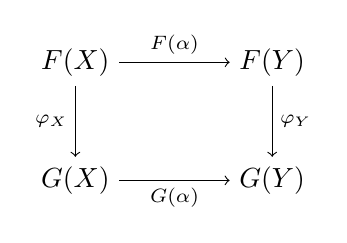
\begin{tikzpicture}
					\node (a) at (0,1.5) {$F(X)$};
					\node (b)at (2.5,1.5) {$F(Y)$};
					\node (c) at (0,0) {$G(X)$};
					\node (d) at (2.5,0) {$G(Y)$};
					\scriptsize
					\draw[->] (a) -- (b) node[pos=0.5, above] {$F(\alpha)$};
					\draw[->] (c) -- (d) node[pos=0.5, below] {$G(\alpha)$};
					\draw[->] (a) -- (c) node[pos=0.5, left] {$\phi_X$};
					\draw[->] (b) -- (d) node[pos=0.5, right] {$\phi_Y$};
					\end{tikzpicture}
					
					(if $F,G$ are covariant)
				\end{minipage}
				resp.
				\begin{minipage}{0.35\textwidth}
					\centering
					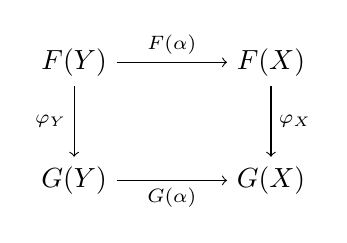
\begin{tikzpicture}
					\node (a) at (0,1.5) {$F(Y)$};
					\node (b)at (2.5,1.5) {$F(X)$};
					\node (c) at (0,0) {$G(Y)$};
					\node (d) at (2.5,0) {$G(X)$};
					\scriptsize
					\draw[->] (a) -- (b) node[pos=0.5, above] {$F(\alpha)$};
					\draw[->] (c) -- (d) node[pos=0.5, below] {$G(\alpha)$};
					\draw[->] (a) -- (c) node[pos=0.5, left] {$\phi_Y$};
					\draw[->] (b) -- (d) node[pos=0.5, right] {$\phi_X$};
					\end{tikzpicture}
					
					(if $F,G$ are contravariant)
				\end{minipage}
			\end{center}
			commutes. If $F\morphism[\phi]G\morphism[\psi]H$ are functormorphisms, then so is $F\morphism[\psi\circ\phi]H$ defined by $(\psi\circ\phi)_X=\psi_X\circ\phi_X$. Obviously, there is a functormorphism $F\morphism[\id_F]F$ given by $\left(\id_F\right)_X=\id_F(X)$. We thus have a \emph{category} of co- resp. contravariant functors $\Aa\morphism[F]\Bb$ between given categories $\Aa,\Bb$.
		\end{alphanumerate}
	\end{rem*}









\end{document}

